\def\secforfig{appendices/lowptcat}
\def\figsversion{V1}


\begin{figure}[ht]
    \centering
    \subfloat{\label{fig:bkgdest16-logpT-1-norw-Control-4bLowPtcat}%
            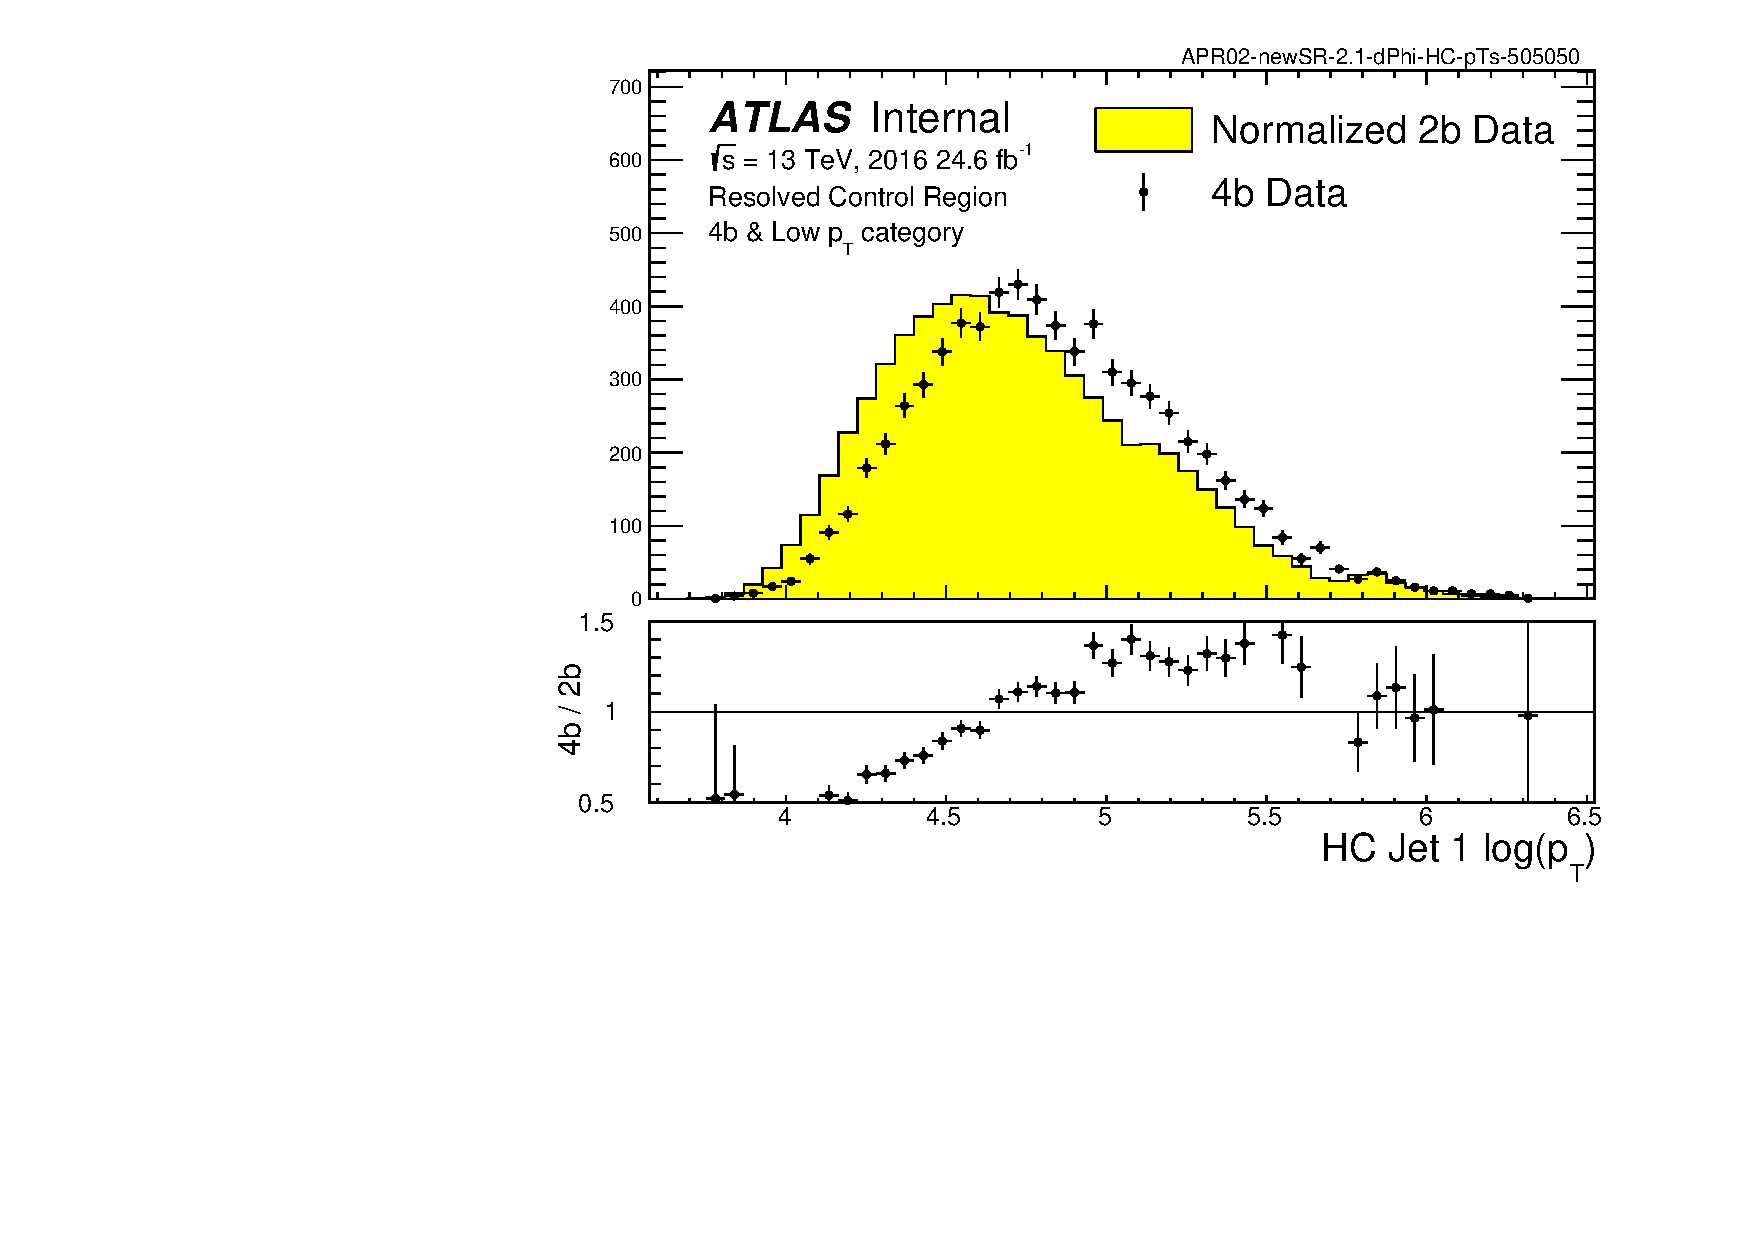
\includegraphics[width=0.4\textwidth]{\figpath{bkgdest-strategy/2016/bkgdest-logpT-1-norw-bstrap-med-shapesyst-Control-4bLowPtcat-NN-16.pdf}}
    }
    \subfloat{\label{fig:bkgdest16-logpT-1-Control-4bLowPtcat}%
            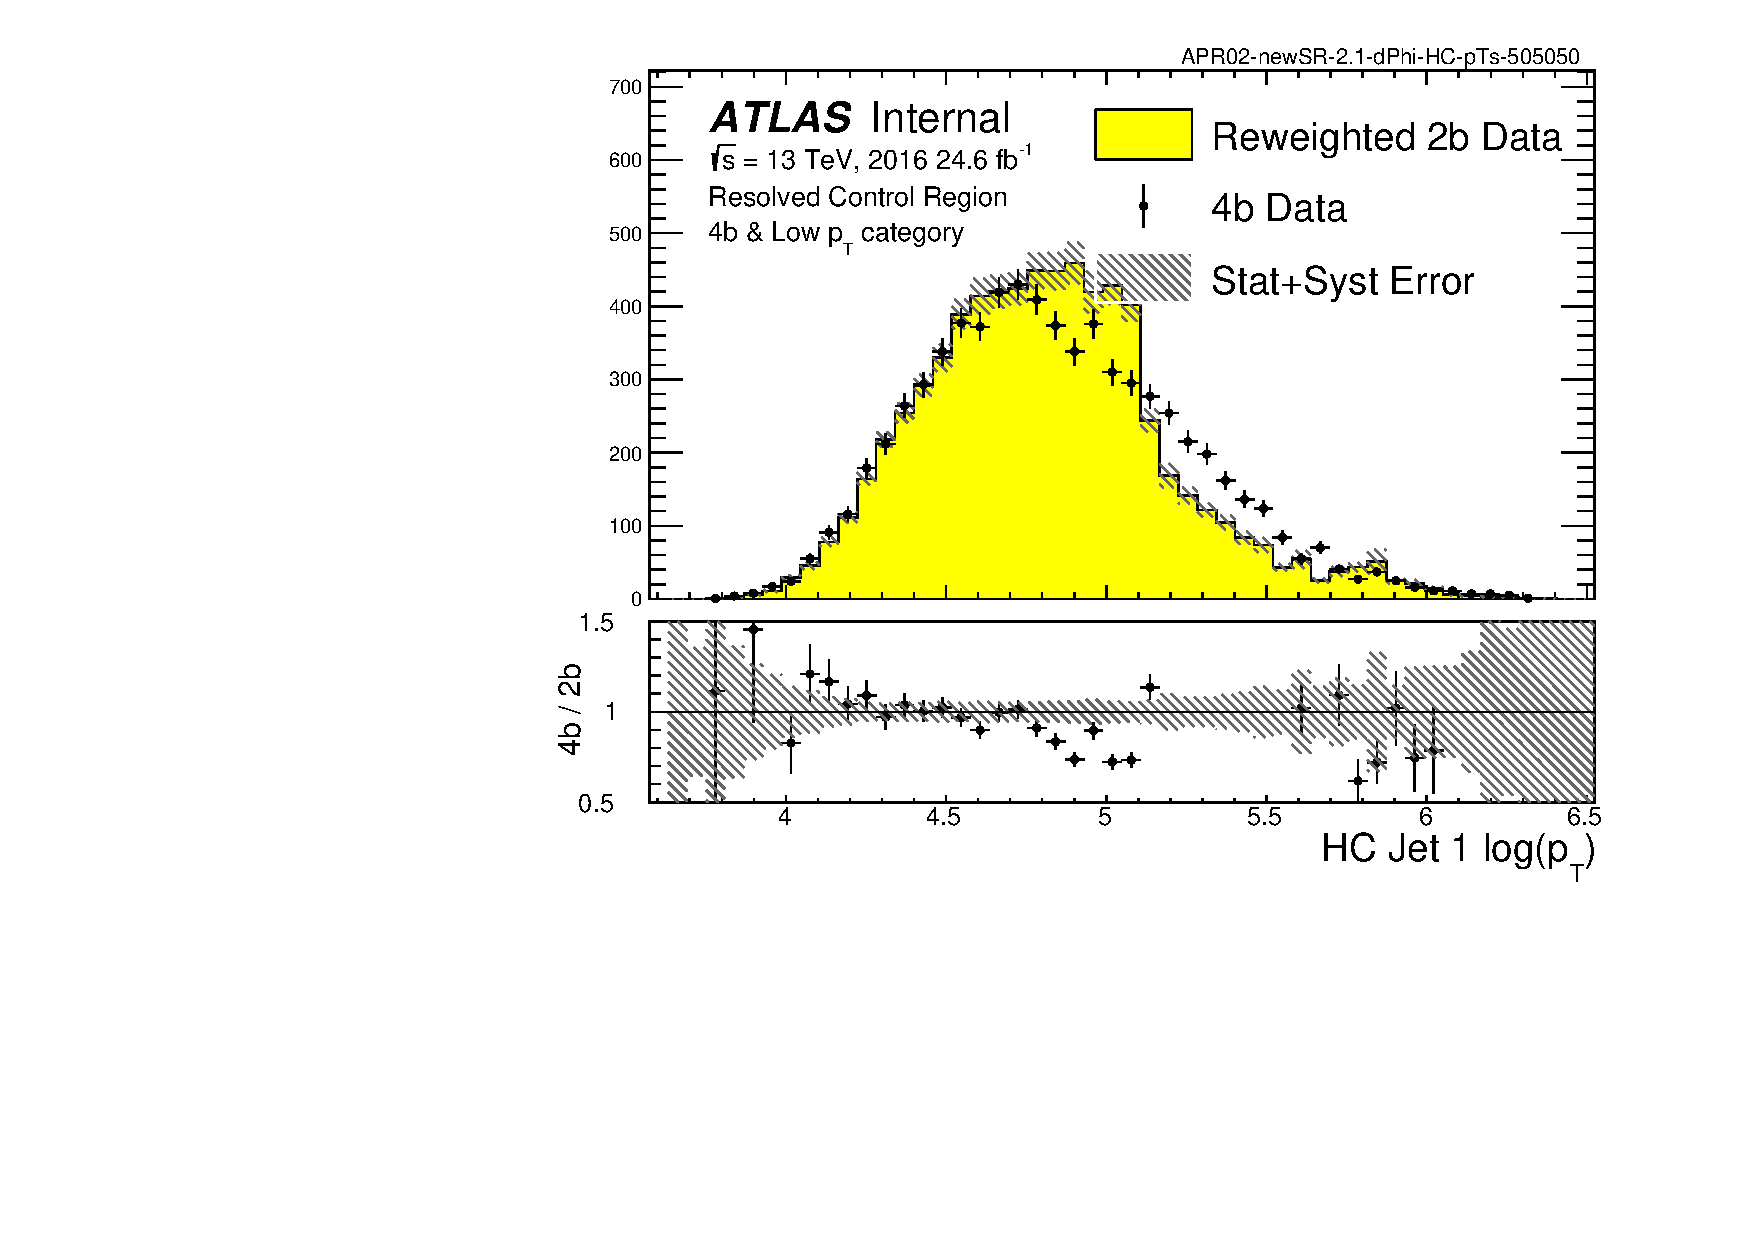
\includegraphics[width=0.4\textwidth]{\figpath{bkgdest-strategy/2016/bkgdest-logpT-1-bstrap-med-shapesyst-Control-4bLowPtcat-NN-16.pdf}}
    }

    \subfloat{\label{fig:bkgdest16-logpT-2-norw-Control-4bLowPtcat}%
            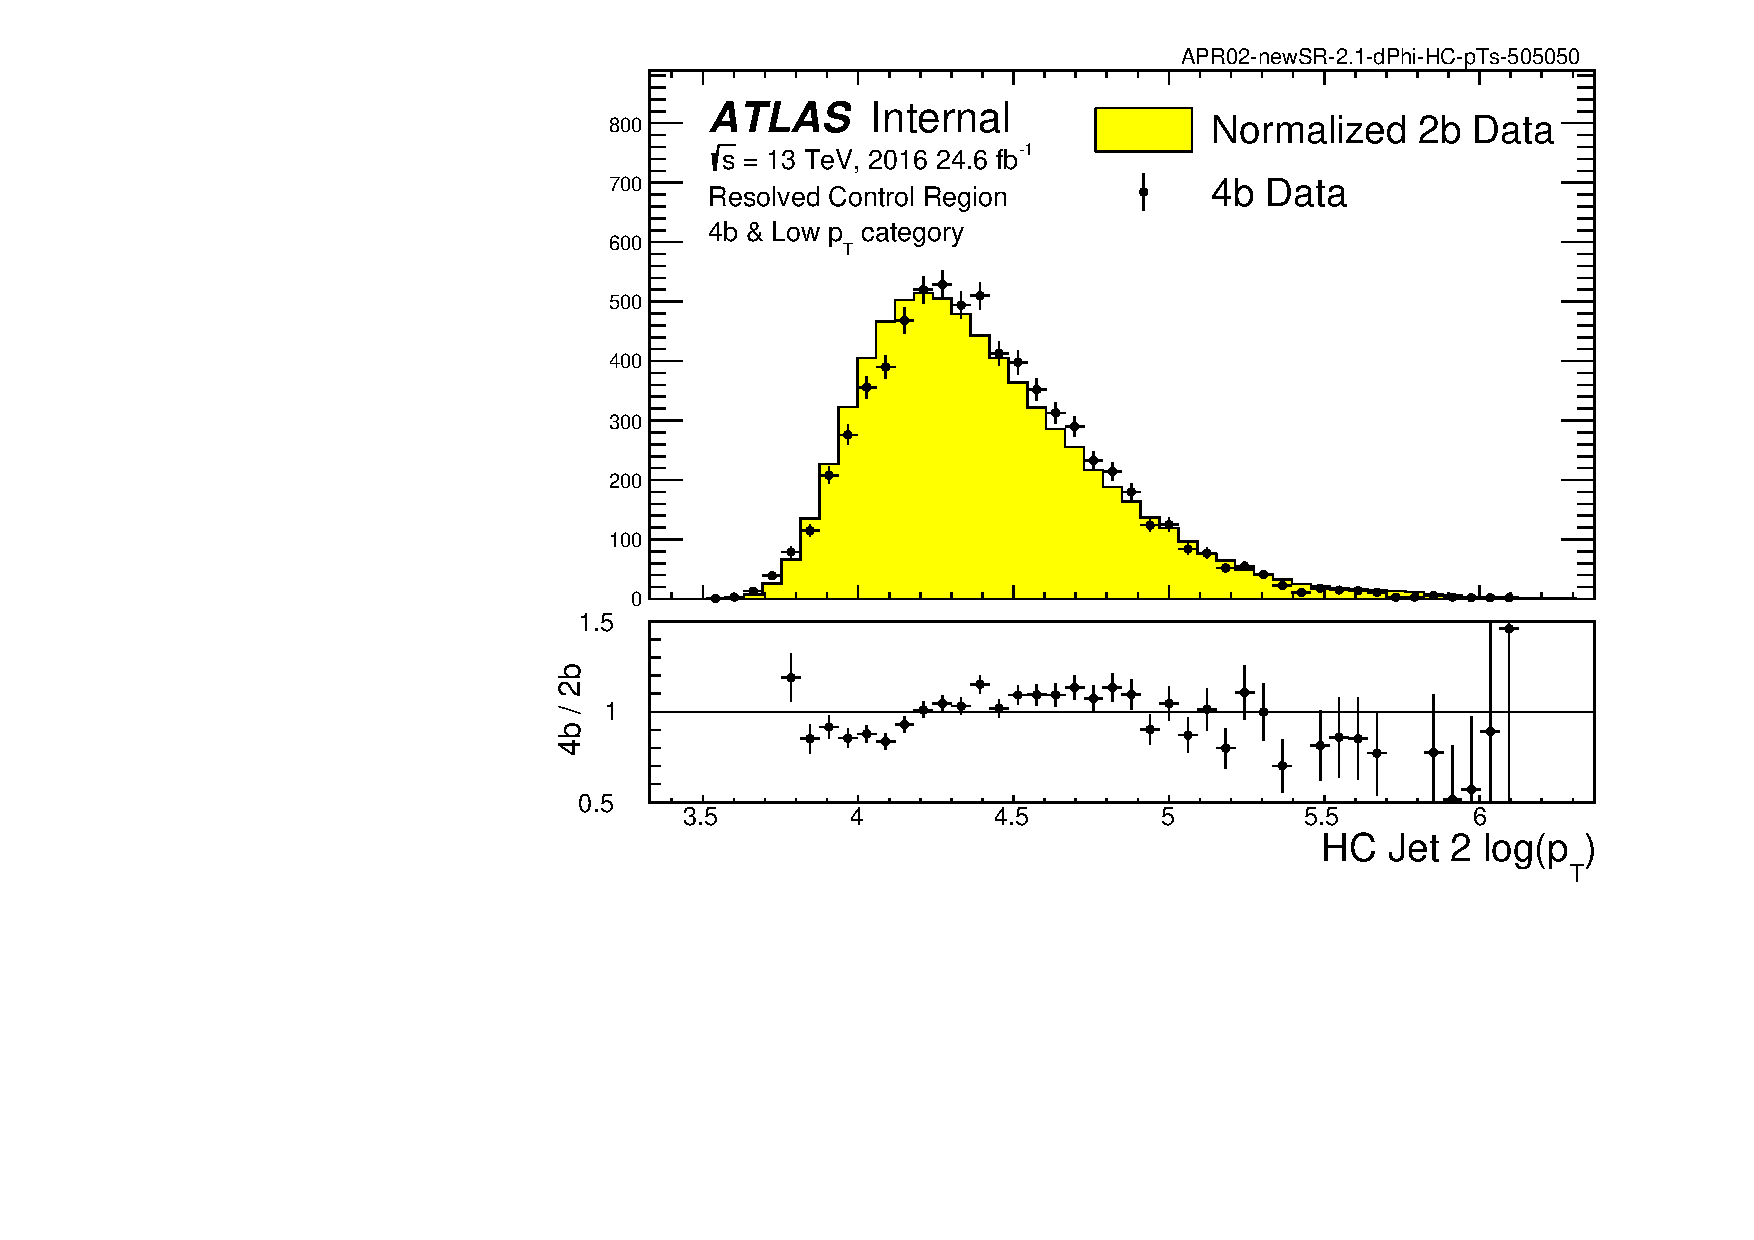
\includegraphics[width=0.4\textwidth]{\figpath{bkgdest-strategy/2016/bkgdest-logpT-2-norw-bstrap-med-shapesyst-Control-4bLowPtcat-NN-16.pdf}}
    }
    \subfloat{\label{fig:bkgdest16-logpT-2-Control-4bLowPtcat}%
            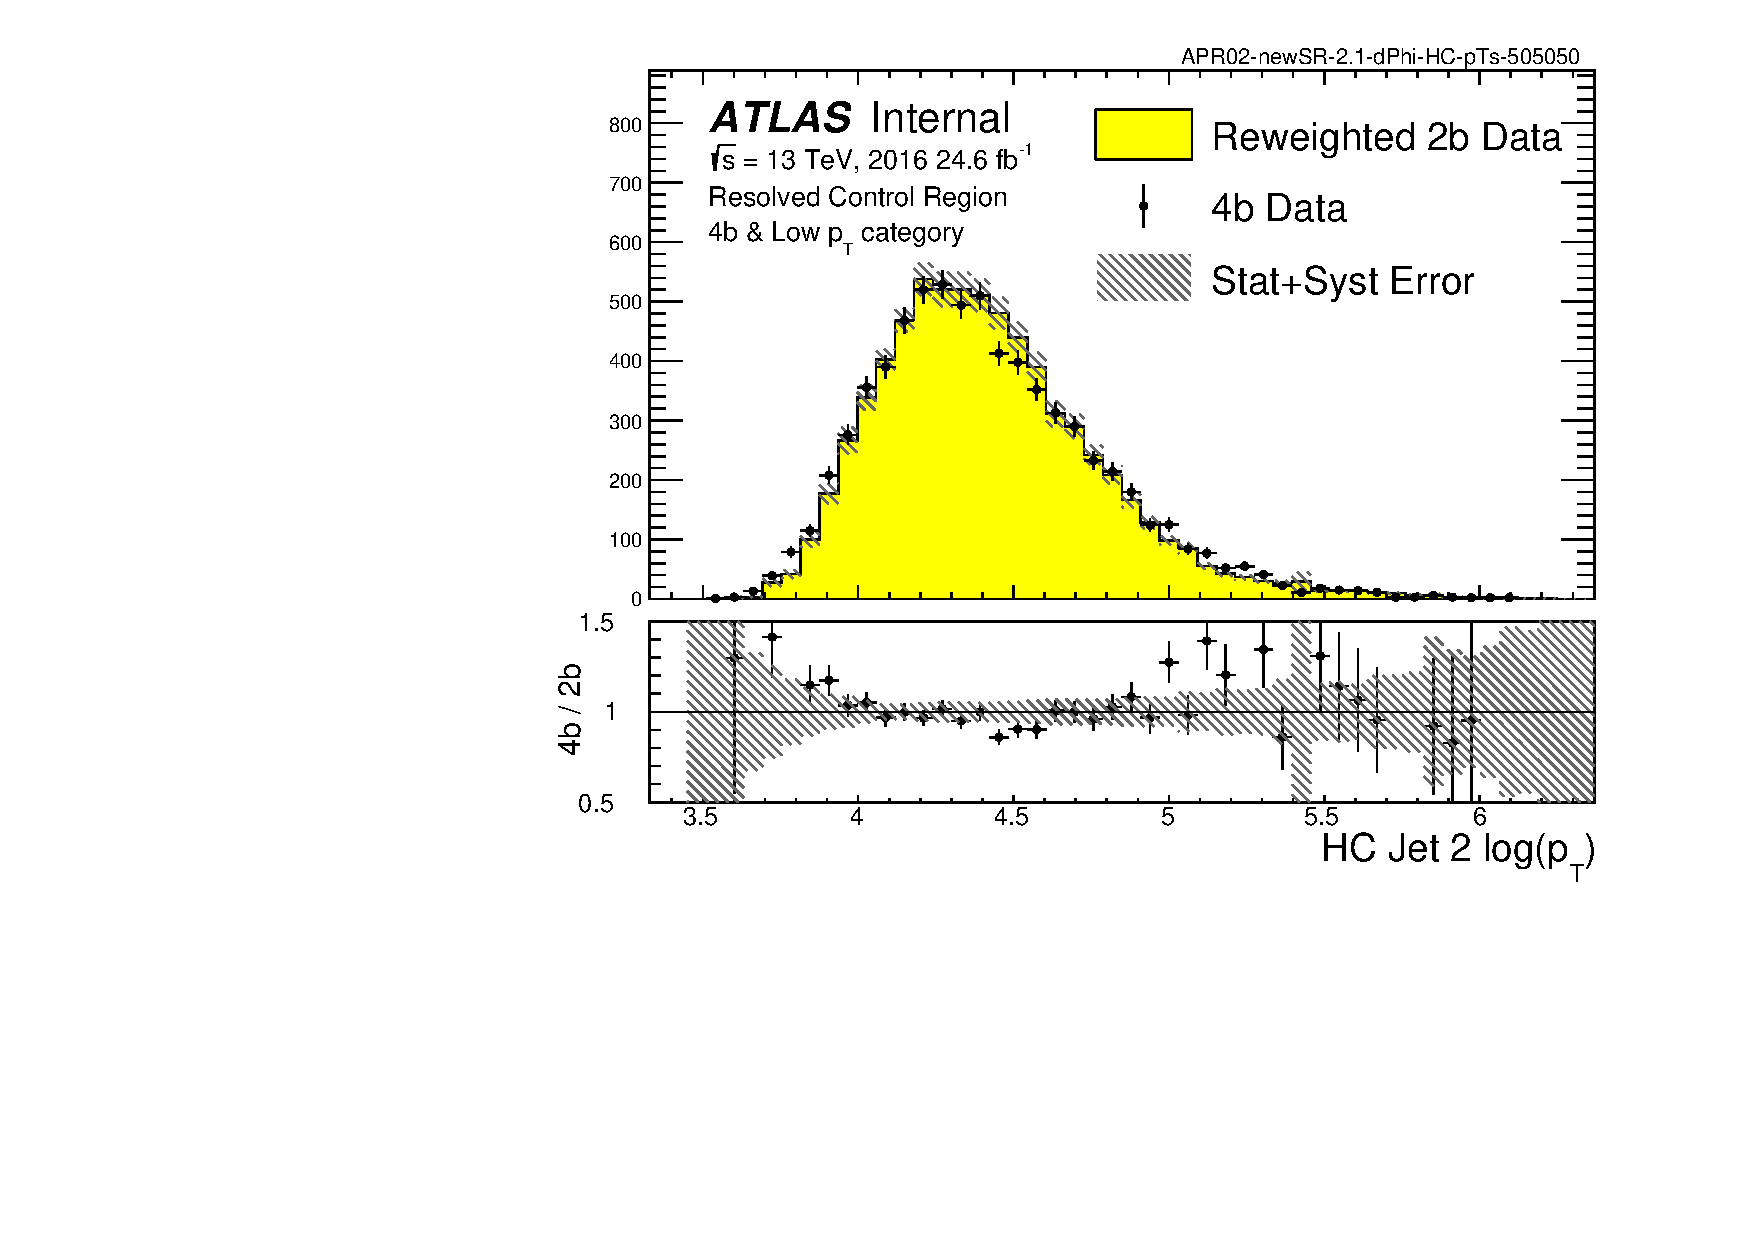
\includegraphics[width=0.4\textwidth]{\figpath{bkgdest-strategy/2016/bkgdest-logpT-2-bstrap-med-shapesyst-Control-4bLowPtcat-NN-16.pdf}}
    }

    \subfloat{\label{fig:bkgdest16-logpT-3-norw-Control-4bLowPtcat}%
            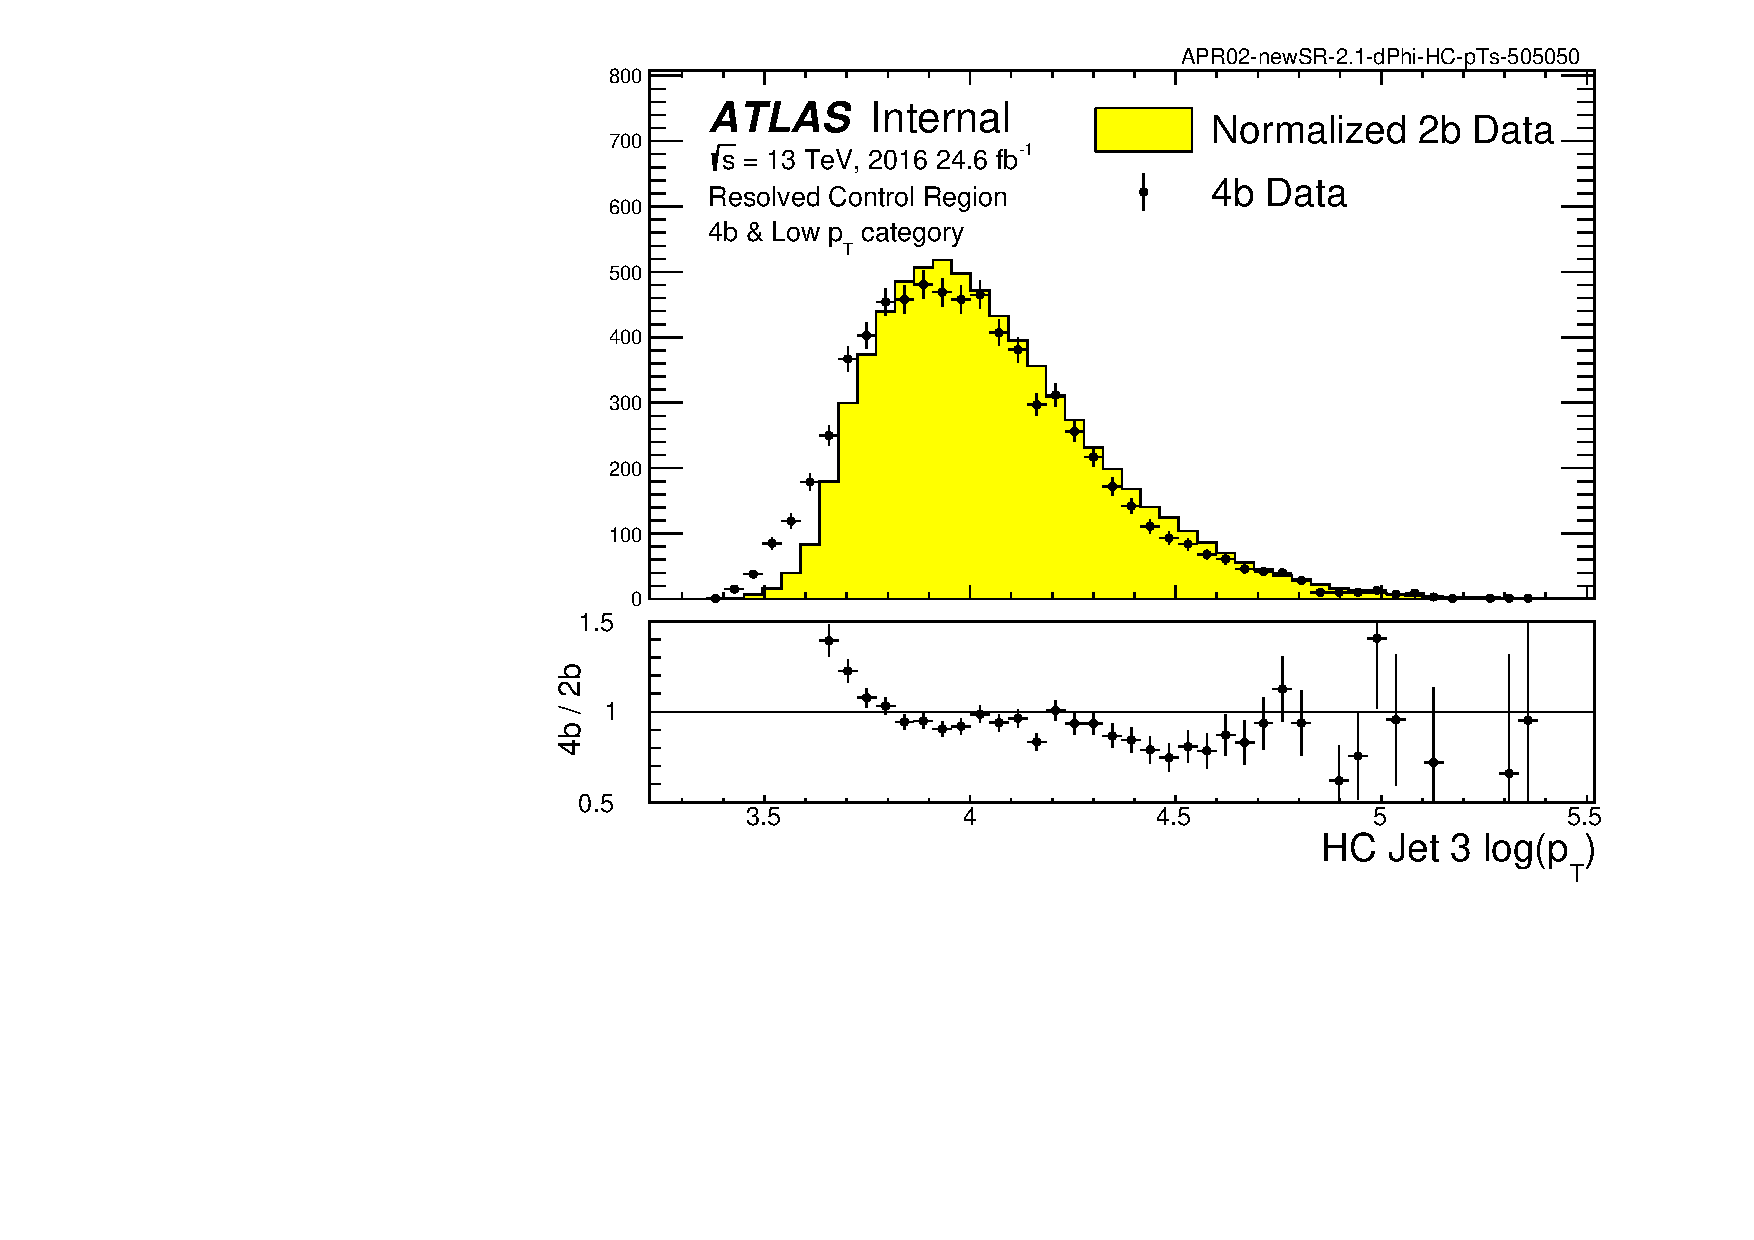
\includegraphics[width=0.4\textwidth]{\figpath{bkgdest-strategy/2016/bkgdest-logpT-3-norw-bstrap-med-shapesyst-Control-4bLowPtcat-NN-16.pdf}}
    }
    \subfloat{\label{fig:bkgdest16-logpT-3-Control-4bLowPtcat}%
            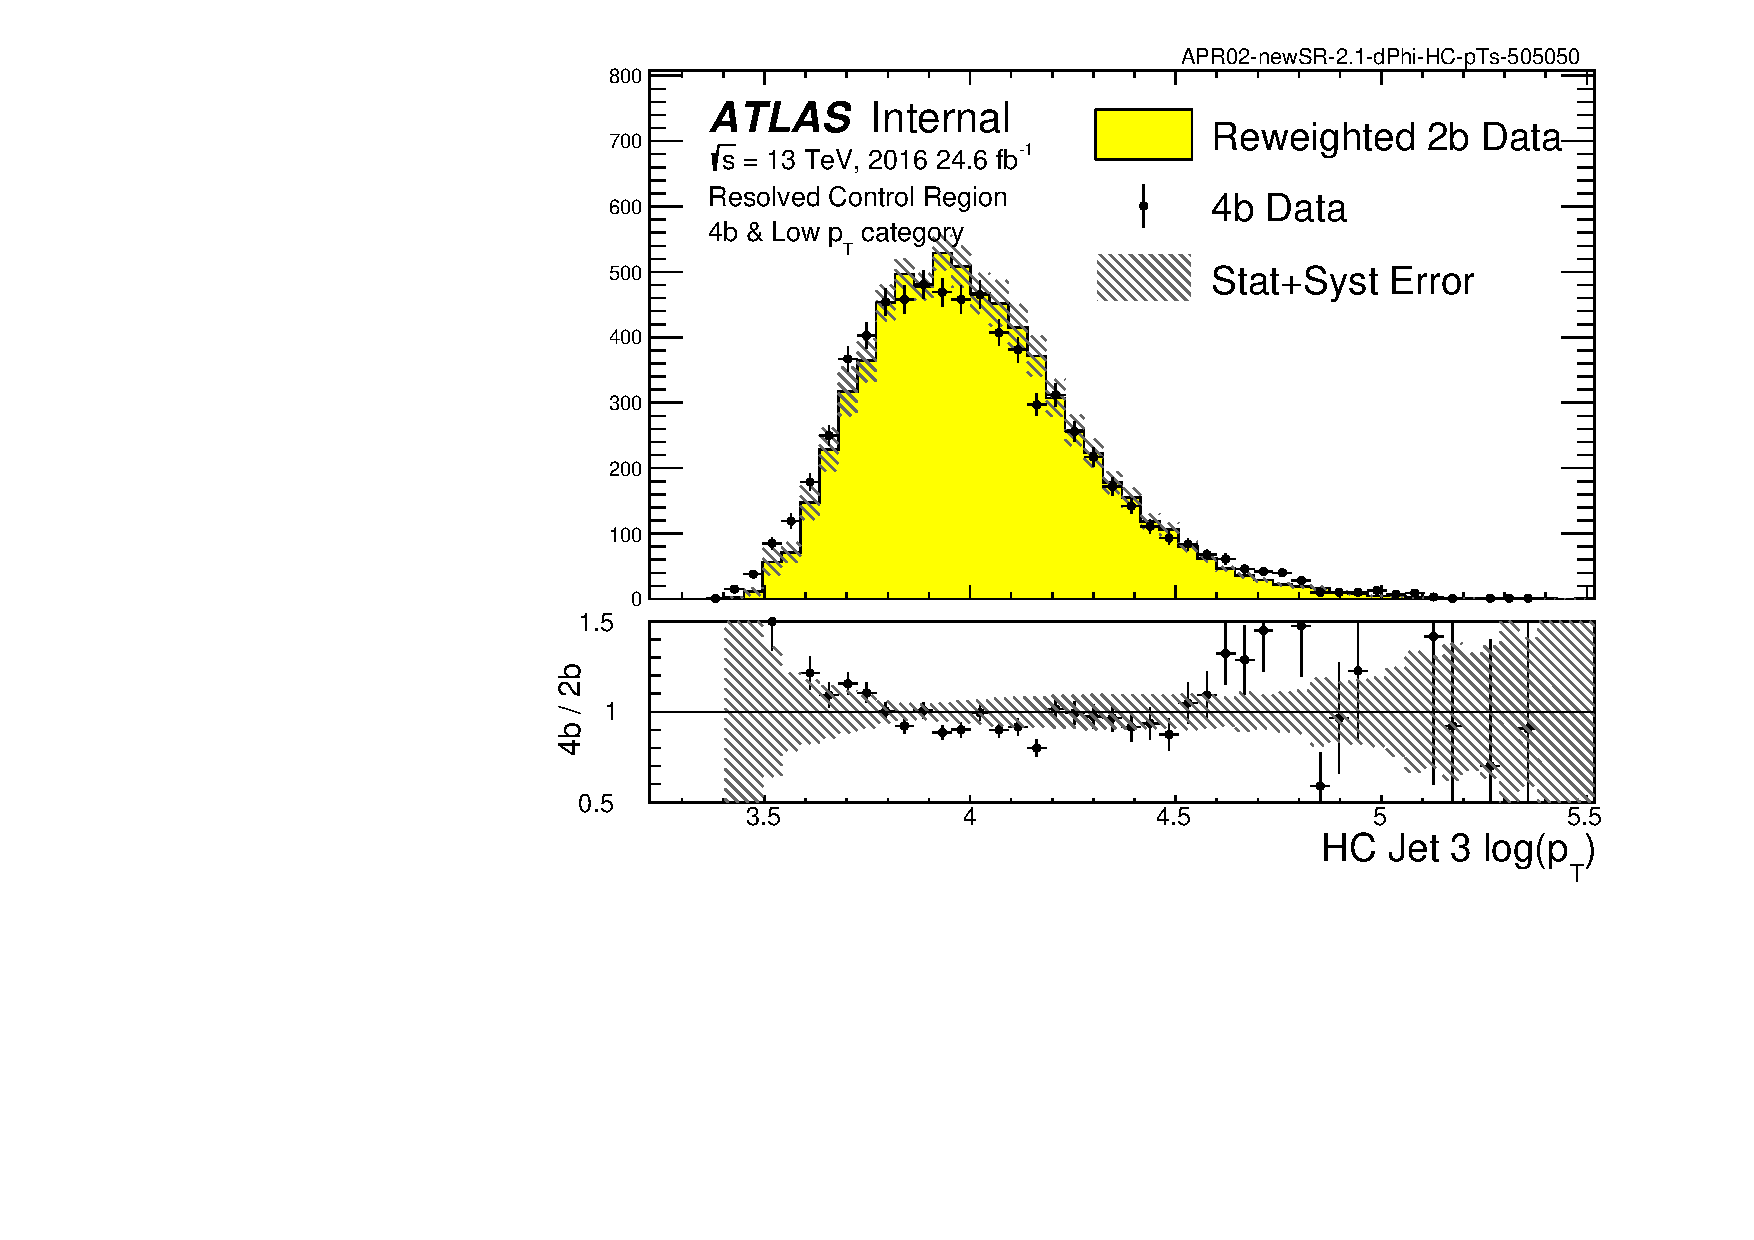
\includegraphics[width=0.4\textwidth]{\figpath{bkgdest-strategy/2016/bkgdest-logpT-3-bstrap-med-shapesyst-Control-4bLowPtcat-NN-16.pdf}}
    }

    \subfloat[Before reweighting]{\label{fig:bkgdest16-logpT-4-norw-Control-4bLowPtcat}%
            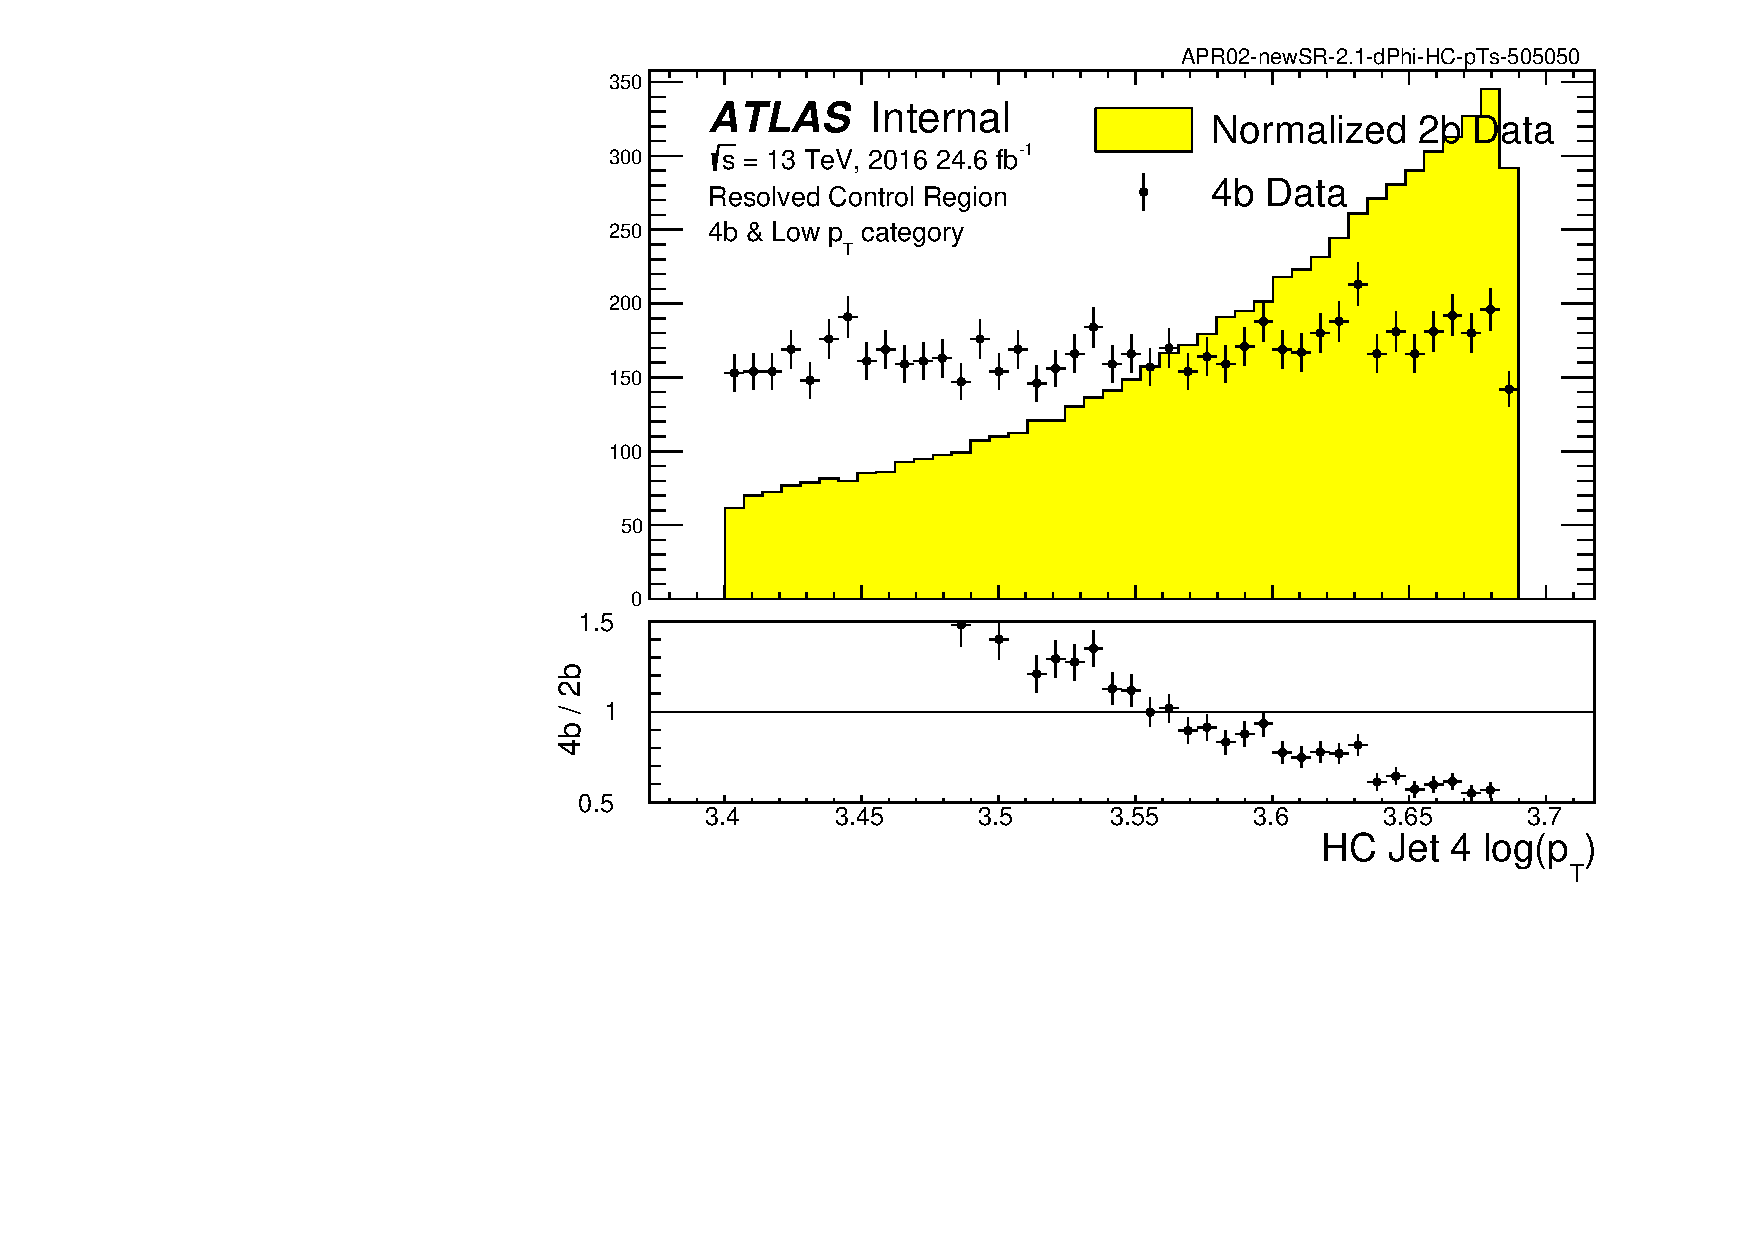
\includegraphics[width=0.4\textwidth]{\figpath{bkgdest-strategy/2016/bkgdest-logpT-4-norw-bstrap-med-shapesyst-Control-4bLowPtcat-NN-16.pdf}}
    }
    \subfloat[After reweighting]{\label{fig:bkgdest16-logpT-4-Control-4bLowPtcat}%
            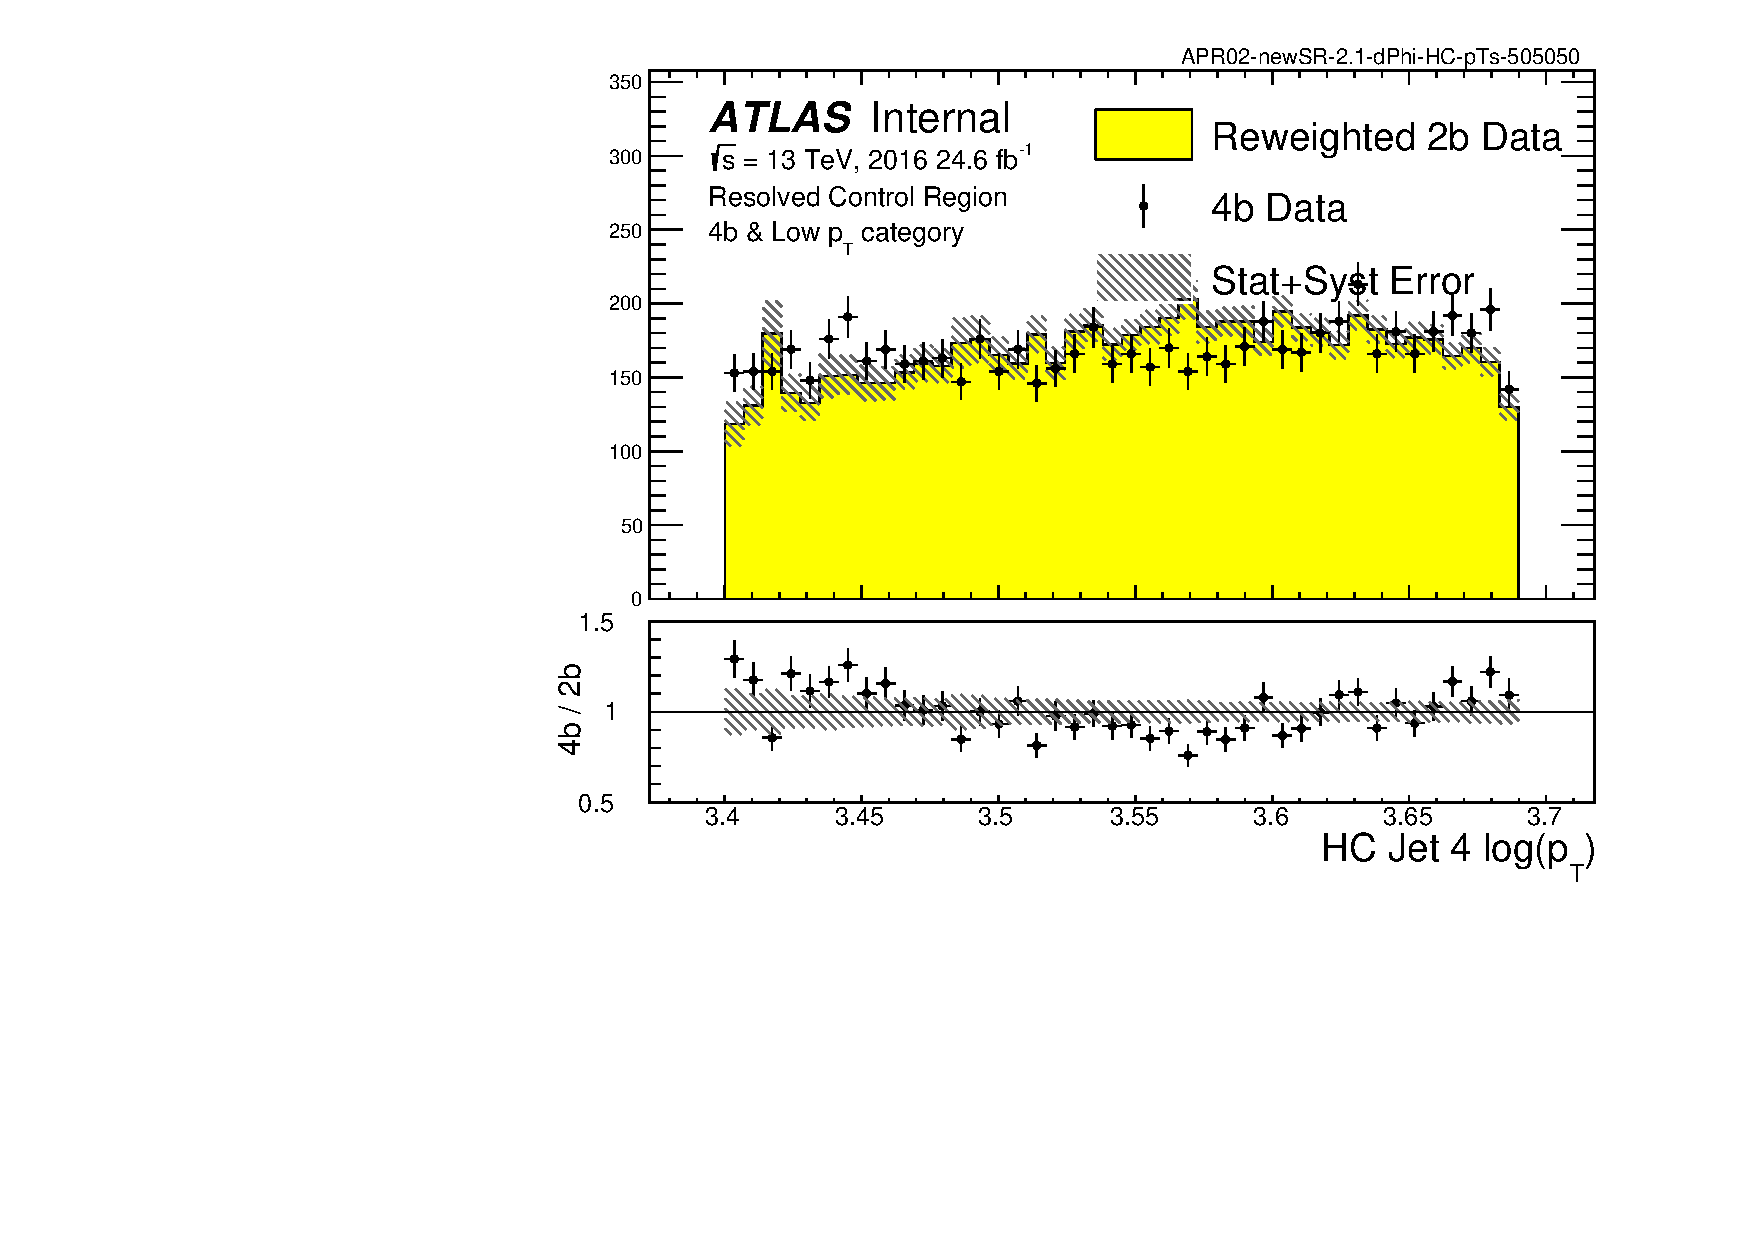
\includegraphics[width=0.4\textwidth]{\figpath{bkgdest-strategy/2016/bkgdest-logpT-4-bstrap-med-shapesyst-Control-4bLowPtcat-NN-16.pdf}}
    }
    \caption{Distributions of log(\pt)-s of the Higgs candidate jets before and after reweighting, which includes log(pt)-s of the 1st and 3rd Higgs candidate jets, in the 2016 Control Region.}
    \label{fig:bkgdest16-1-Control-4bLowPtcat}
\end{figure}


\begin{figure}[ht]
    \centering
    \subfloat{\label{fig:bkgdest16-eta-i-norw-Control-4bLowPtcat}%
            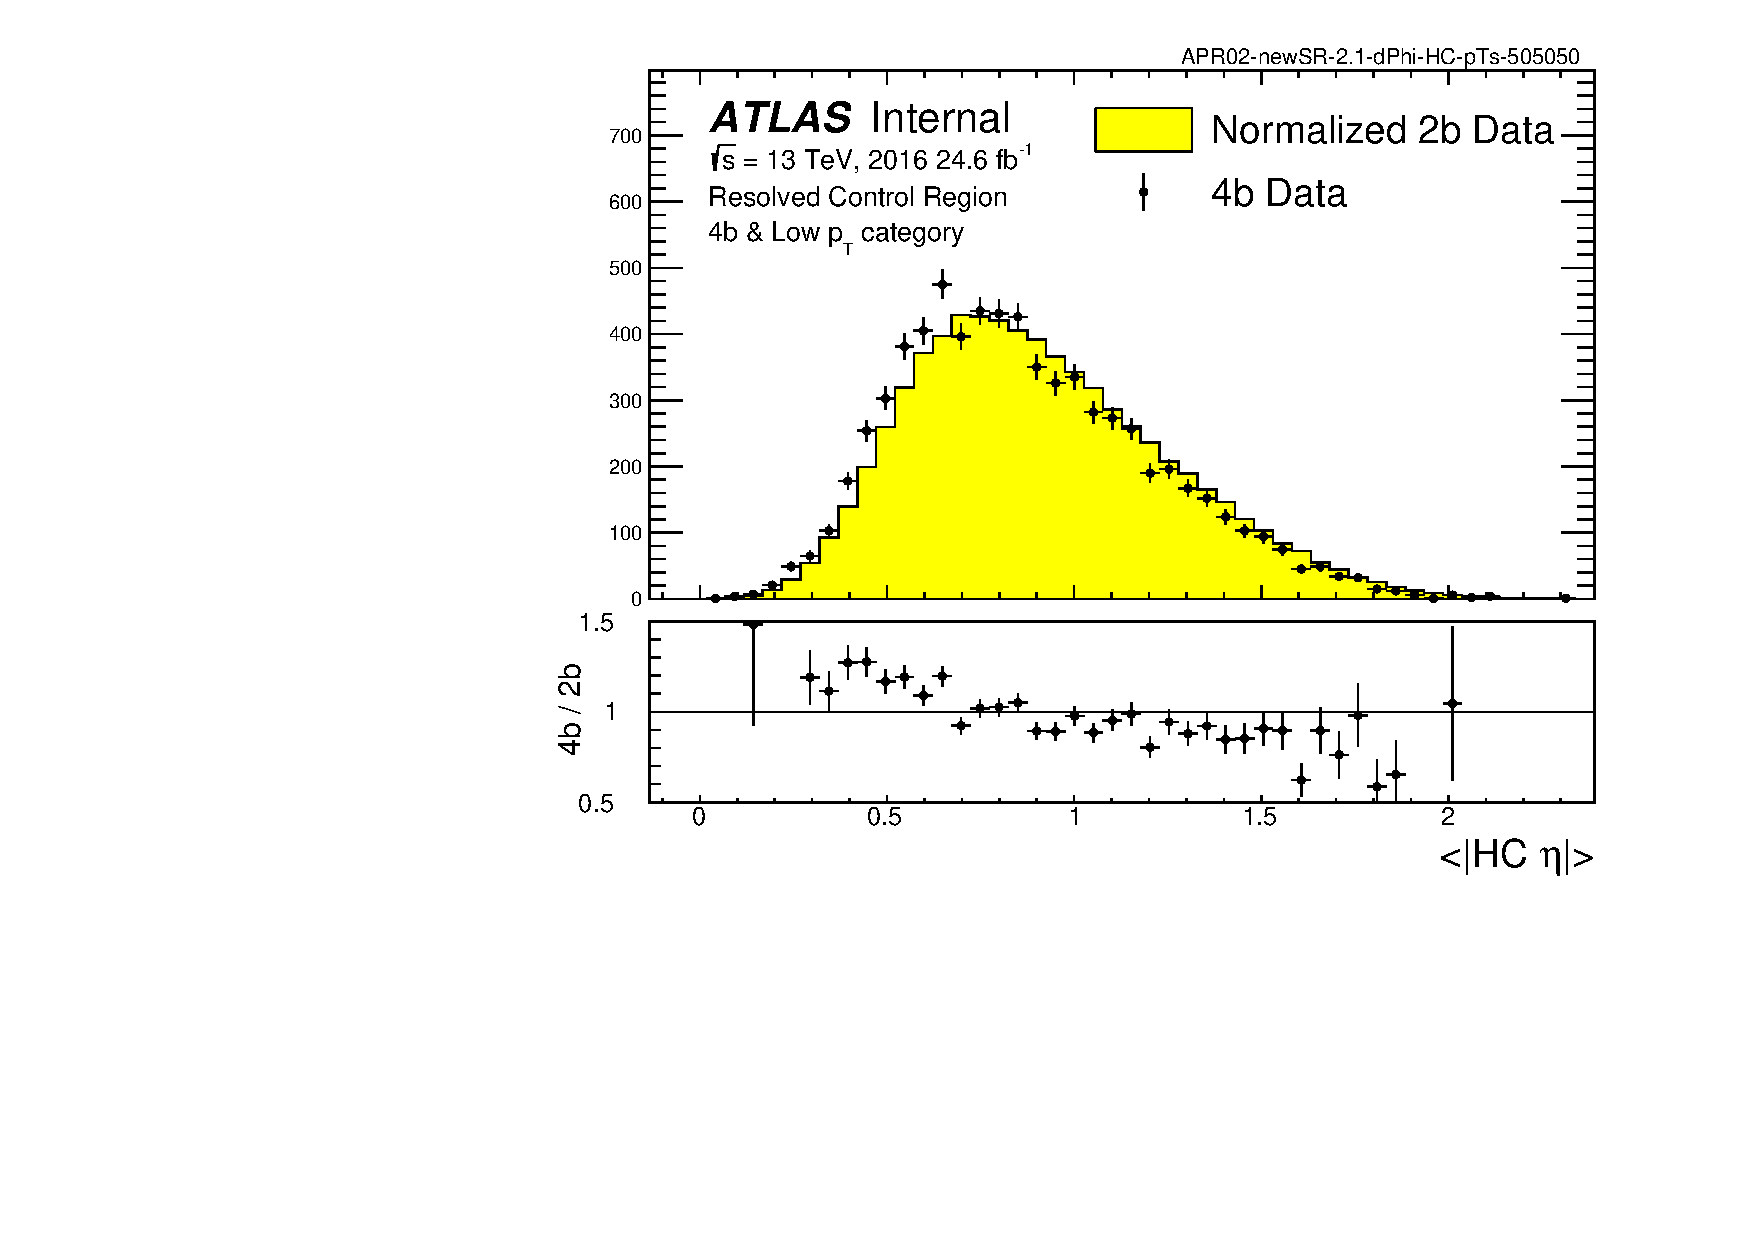
\includegraphics[width=0.4\textwidth]{\figpath{bkgdest-strategy/2016/bkgdest-eta-i-norw-bstrap-med-shapesyst-Control-4bLowPtcat-NN-16.pdf}}
    }
    \subfloat{\label{fig:bkgdest16-eta-i-Control-4bLowPtcat}%
            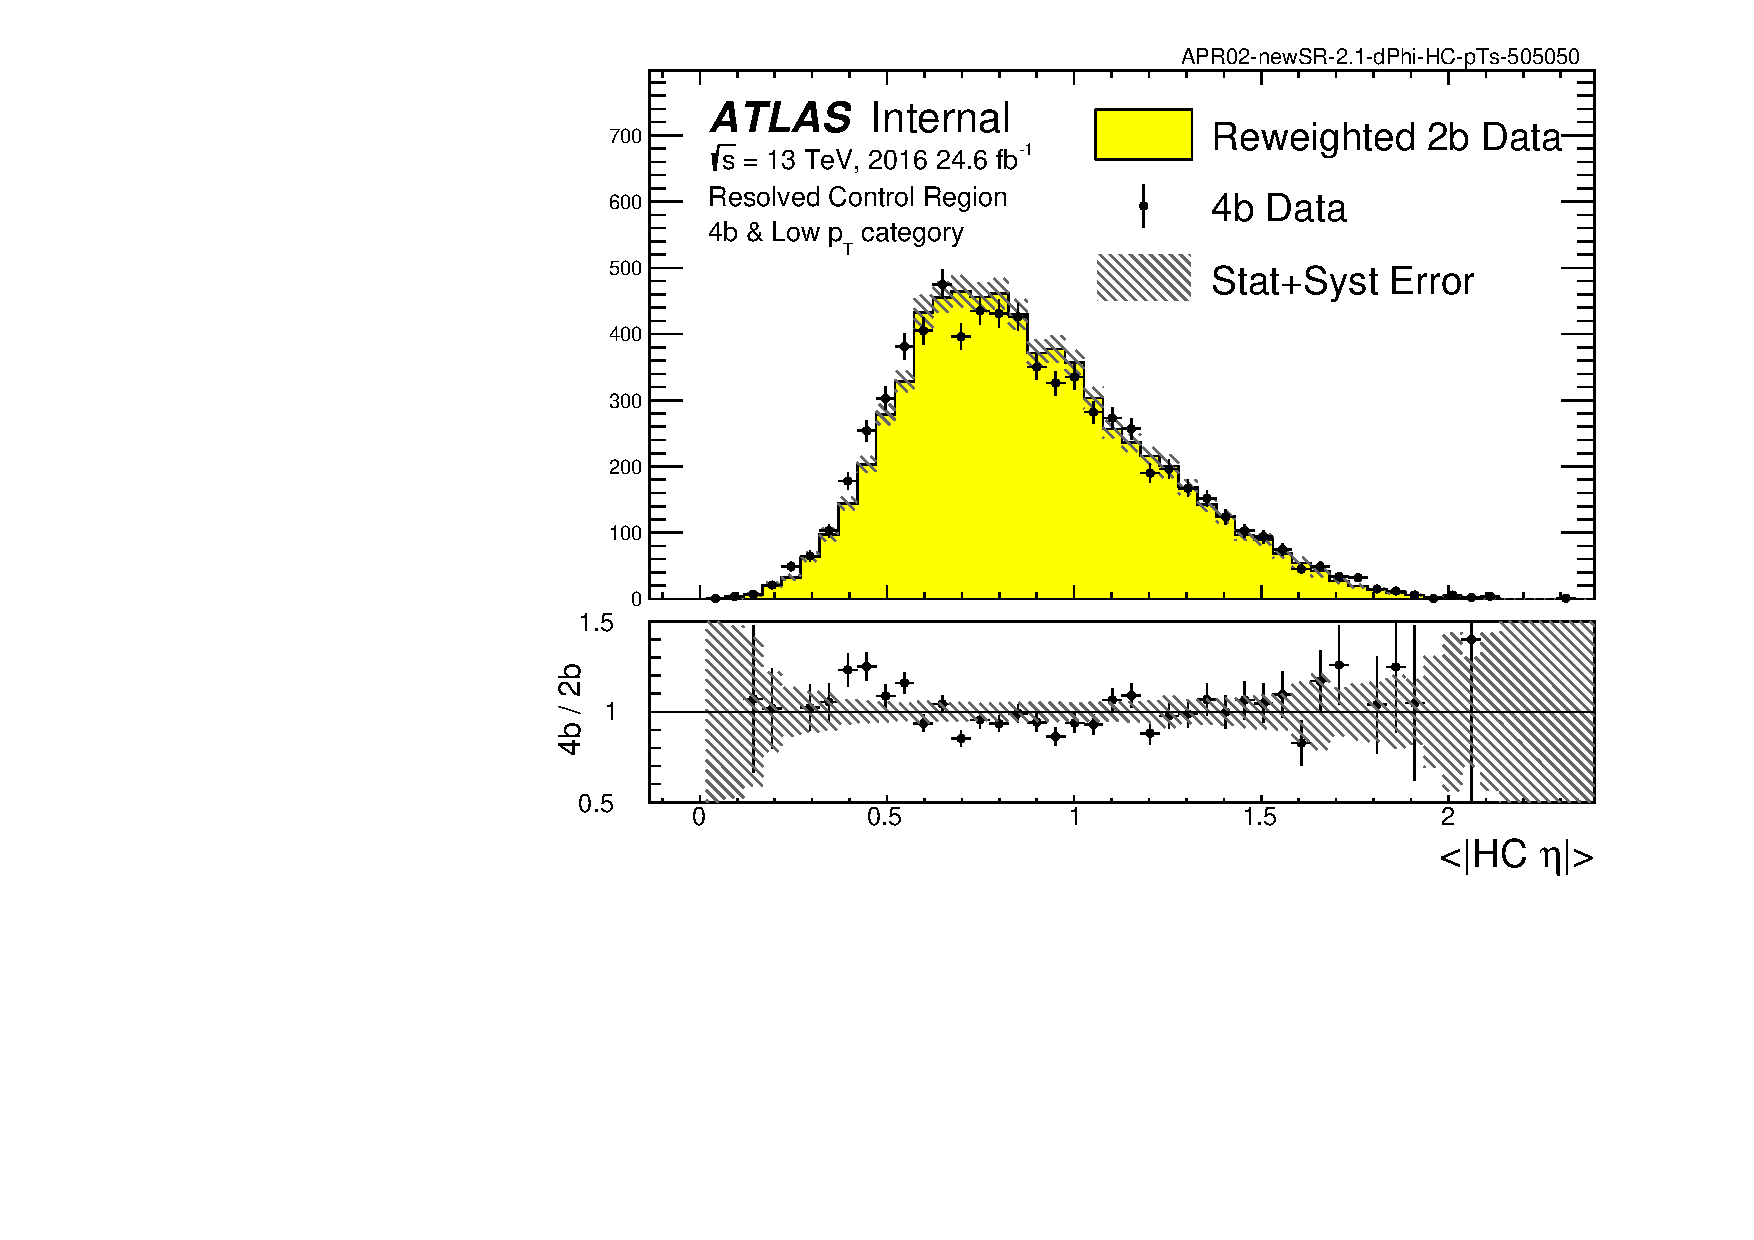
\includegraphics[width=0.4\textwidth]{\figpath{bkgdest-strategy/2016/bkgdest-eta-i-bstrap-med-shapesyst-Control-4bLowPtcat-NN-16.pdf}}
    }

    \subfloat{\label{fig:bkgdest16-dRjj-1-norw-Control-4bLowPtcat}%
            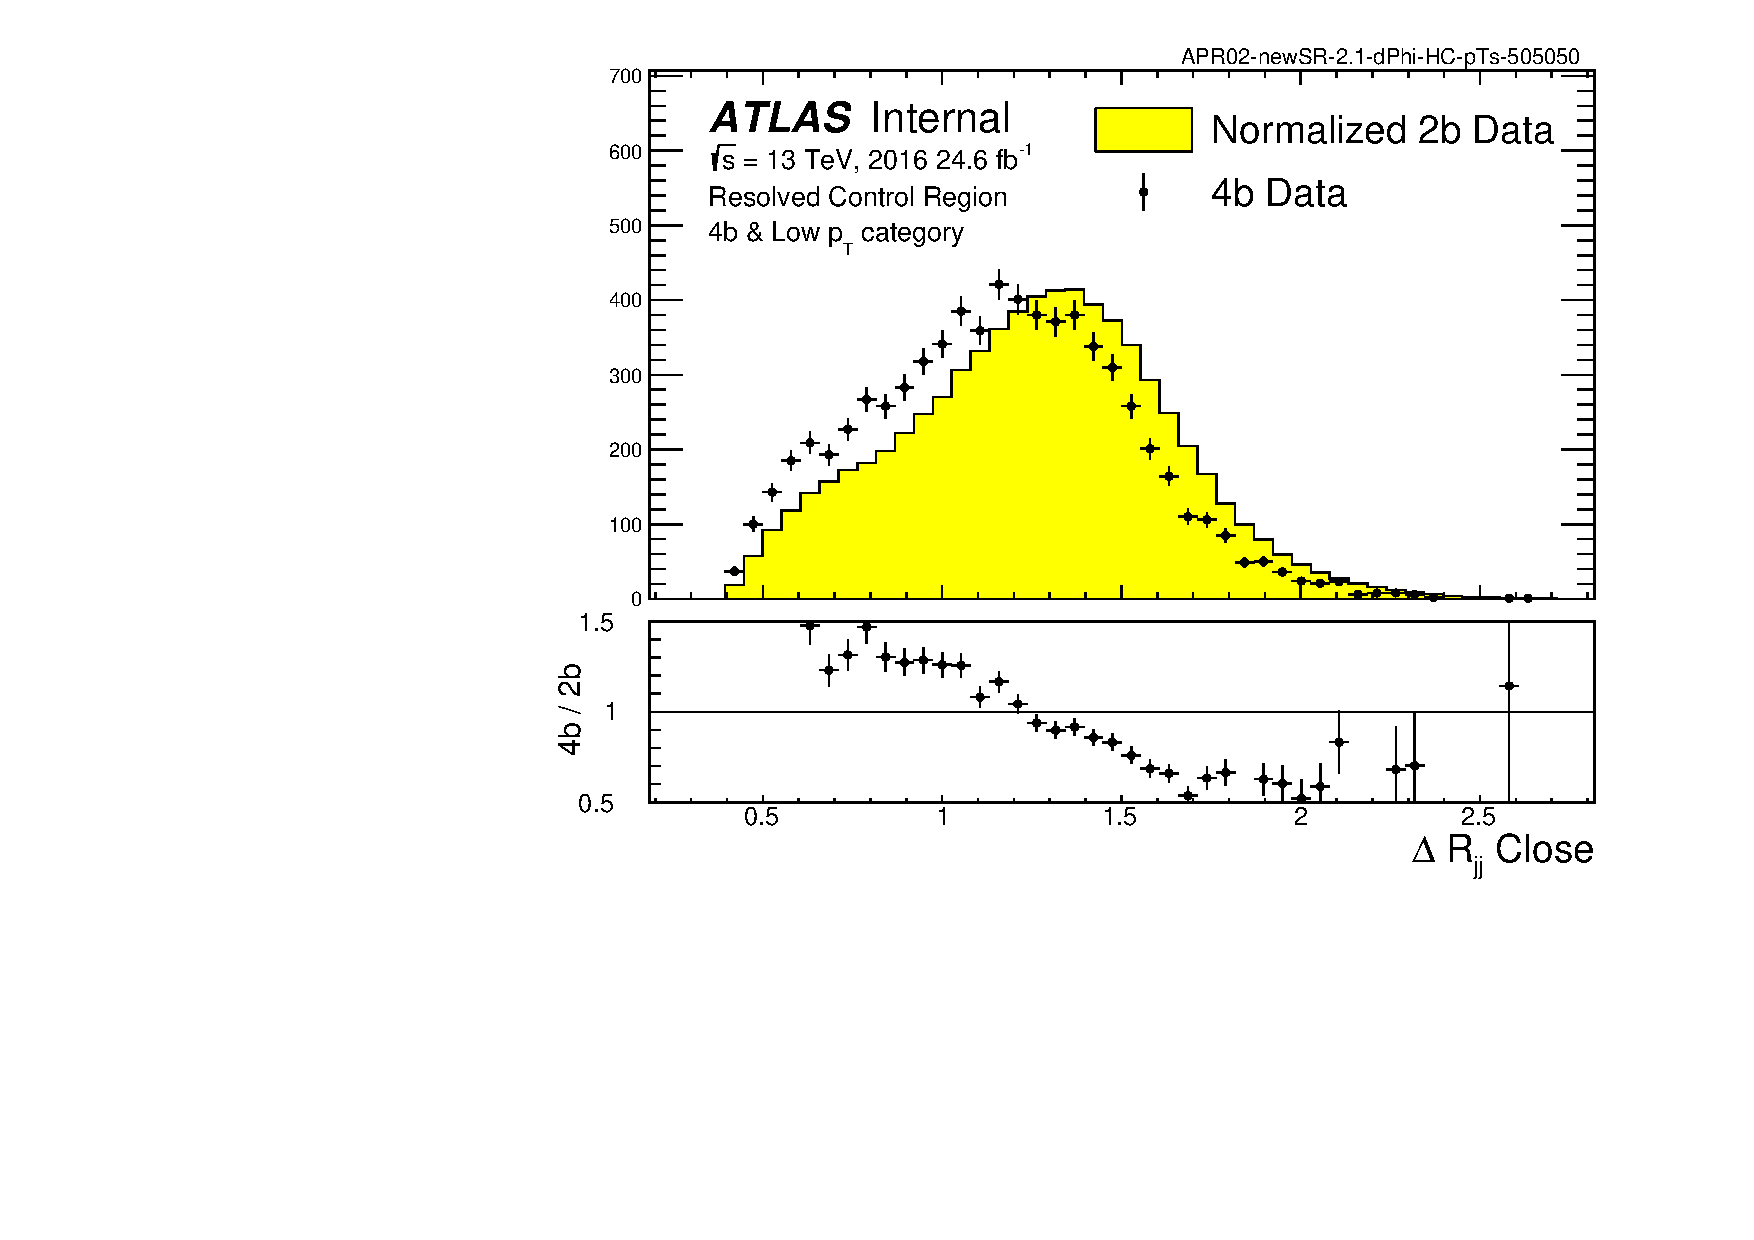
\includegraphics[width=0.4\textwidth]{\figpath{bkgdest-strategy/2016/bkgdest-dRjj-1-norw-bstrap-med-shapesyst-Control-4bLowPtcat-NN-16.pdf}}
    }
    \subfloat{\label{fig:bkgdest16-dRjj-1-Control-4bLowPtcat}%
            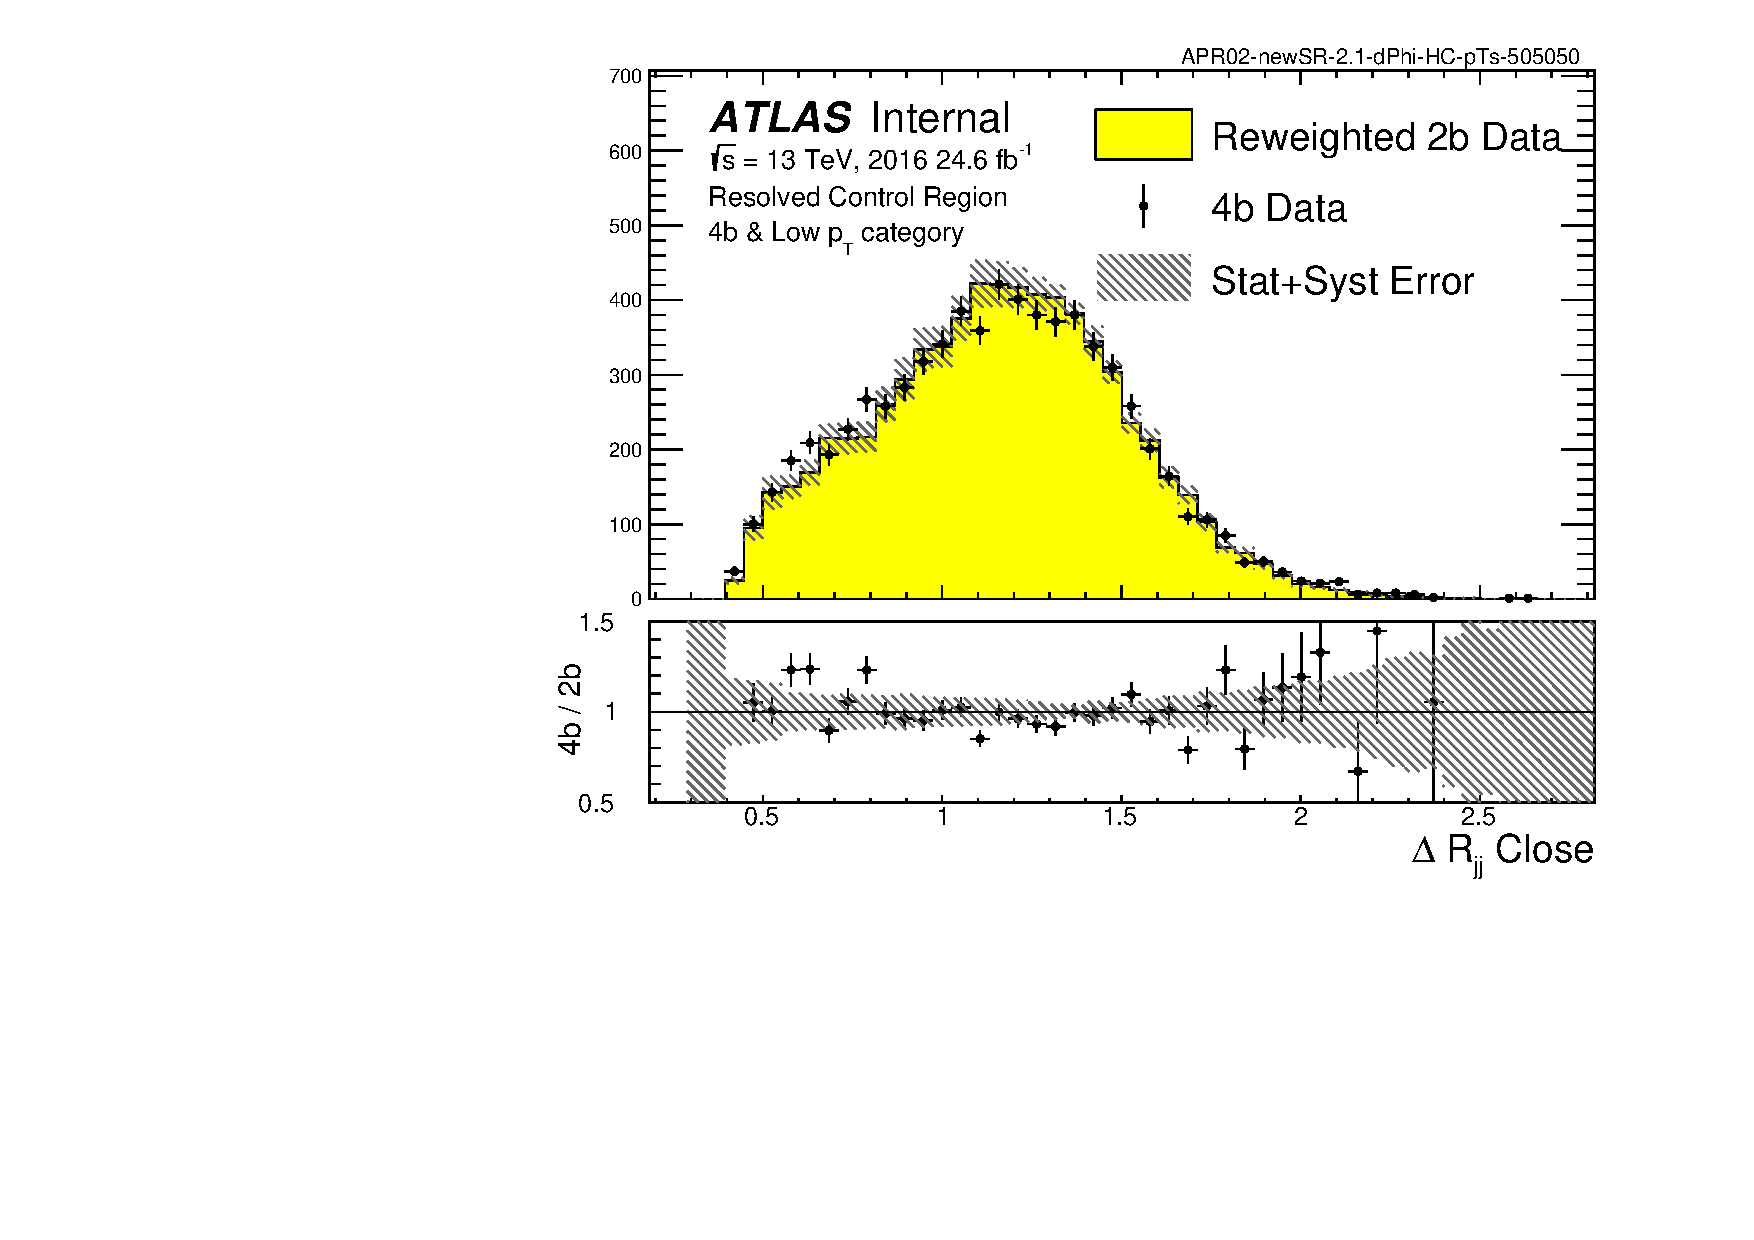
\includegraphics[width=0.4\textwidth]{\figpath{bkgdest-strategy/2016/bkgdest-dRjj-1-bstrap-med-shapesyst-Control-4bLowPtcat-NN-16.pdf}}
    }

    \subfloat[Before reweighting]{\label{fig:bkgdest16-dRjj-2-norw-Control-4bLowPtcat}%
            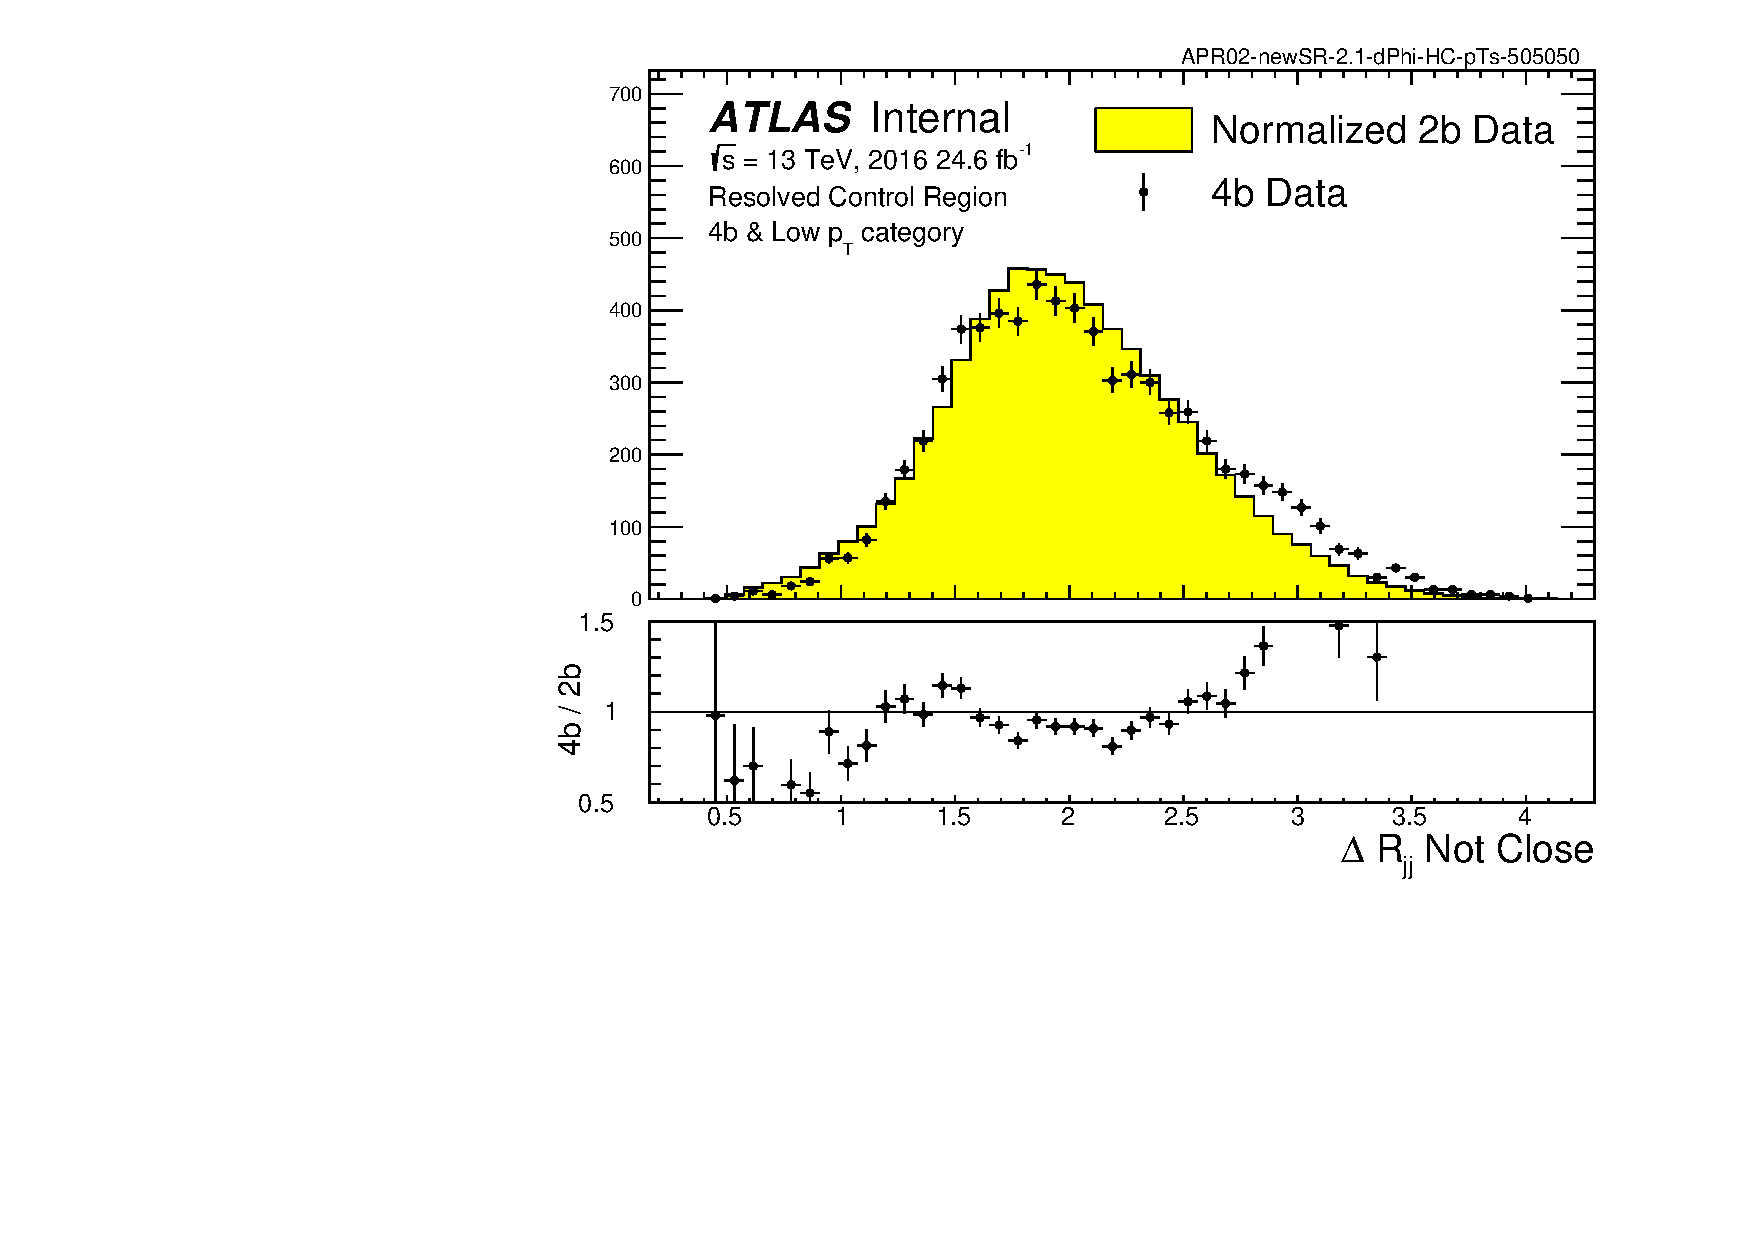
\includegraphics[width=0.4\textwidth]{\figpath{bkgdest-strategy/2016/bkgdest-dRjj-2-norw-bstrap-med-shapesyst-Control-4bLowPtcat-NN-16.pdf}}
    }
    \subfloat[After reweighting]{\label{fig:bkgdest16-dRjj-2-Control-4bLowPtcat}%
            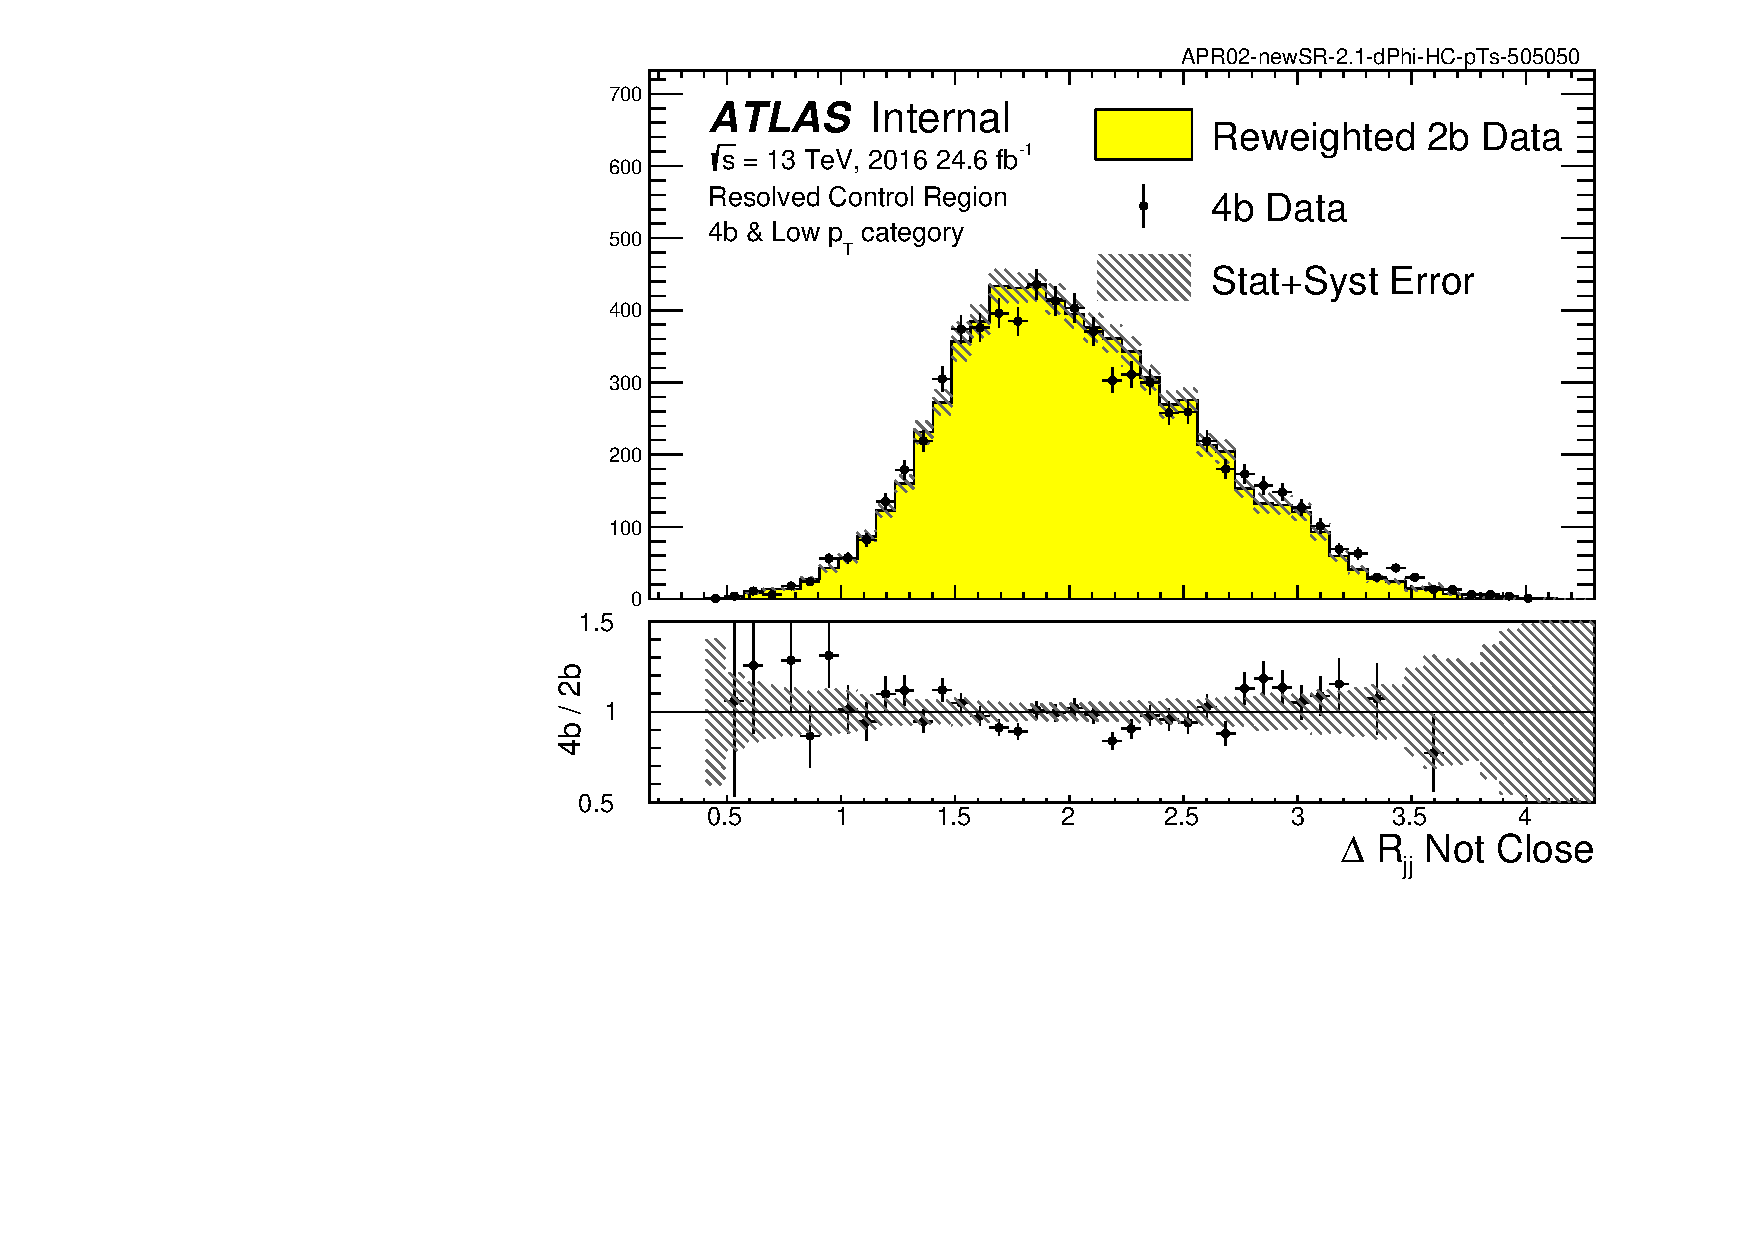
\includegraphics[width=0.4\textwidth]{\figpath{bkgdest-strategy/2016/bkgdest-dRjj-2-bstrap-med-shapesyst-Control-4bLowPtcat-NN-16.pdf}}
    }

    \caption{Distributions of average absolute value of Higgs candidate jet $\eta$ and log(\dr)-s between the closest two Higgs candidate jets and the other two Higgs candidate jets before and after reweighting, which includes log(pt)-s of the 1st and 3rd Higgs candidate jets, in the 2016 Control Region.}
    \label{fig:bkgdest16-2-Control-4bLowPtcat}
\end{figure}


\begin{figure}[ht]
    \centering
    \subfloat{\label{fig:bkgdest16-dPhi-h1-norw-Control-4bLowPtcat}%
            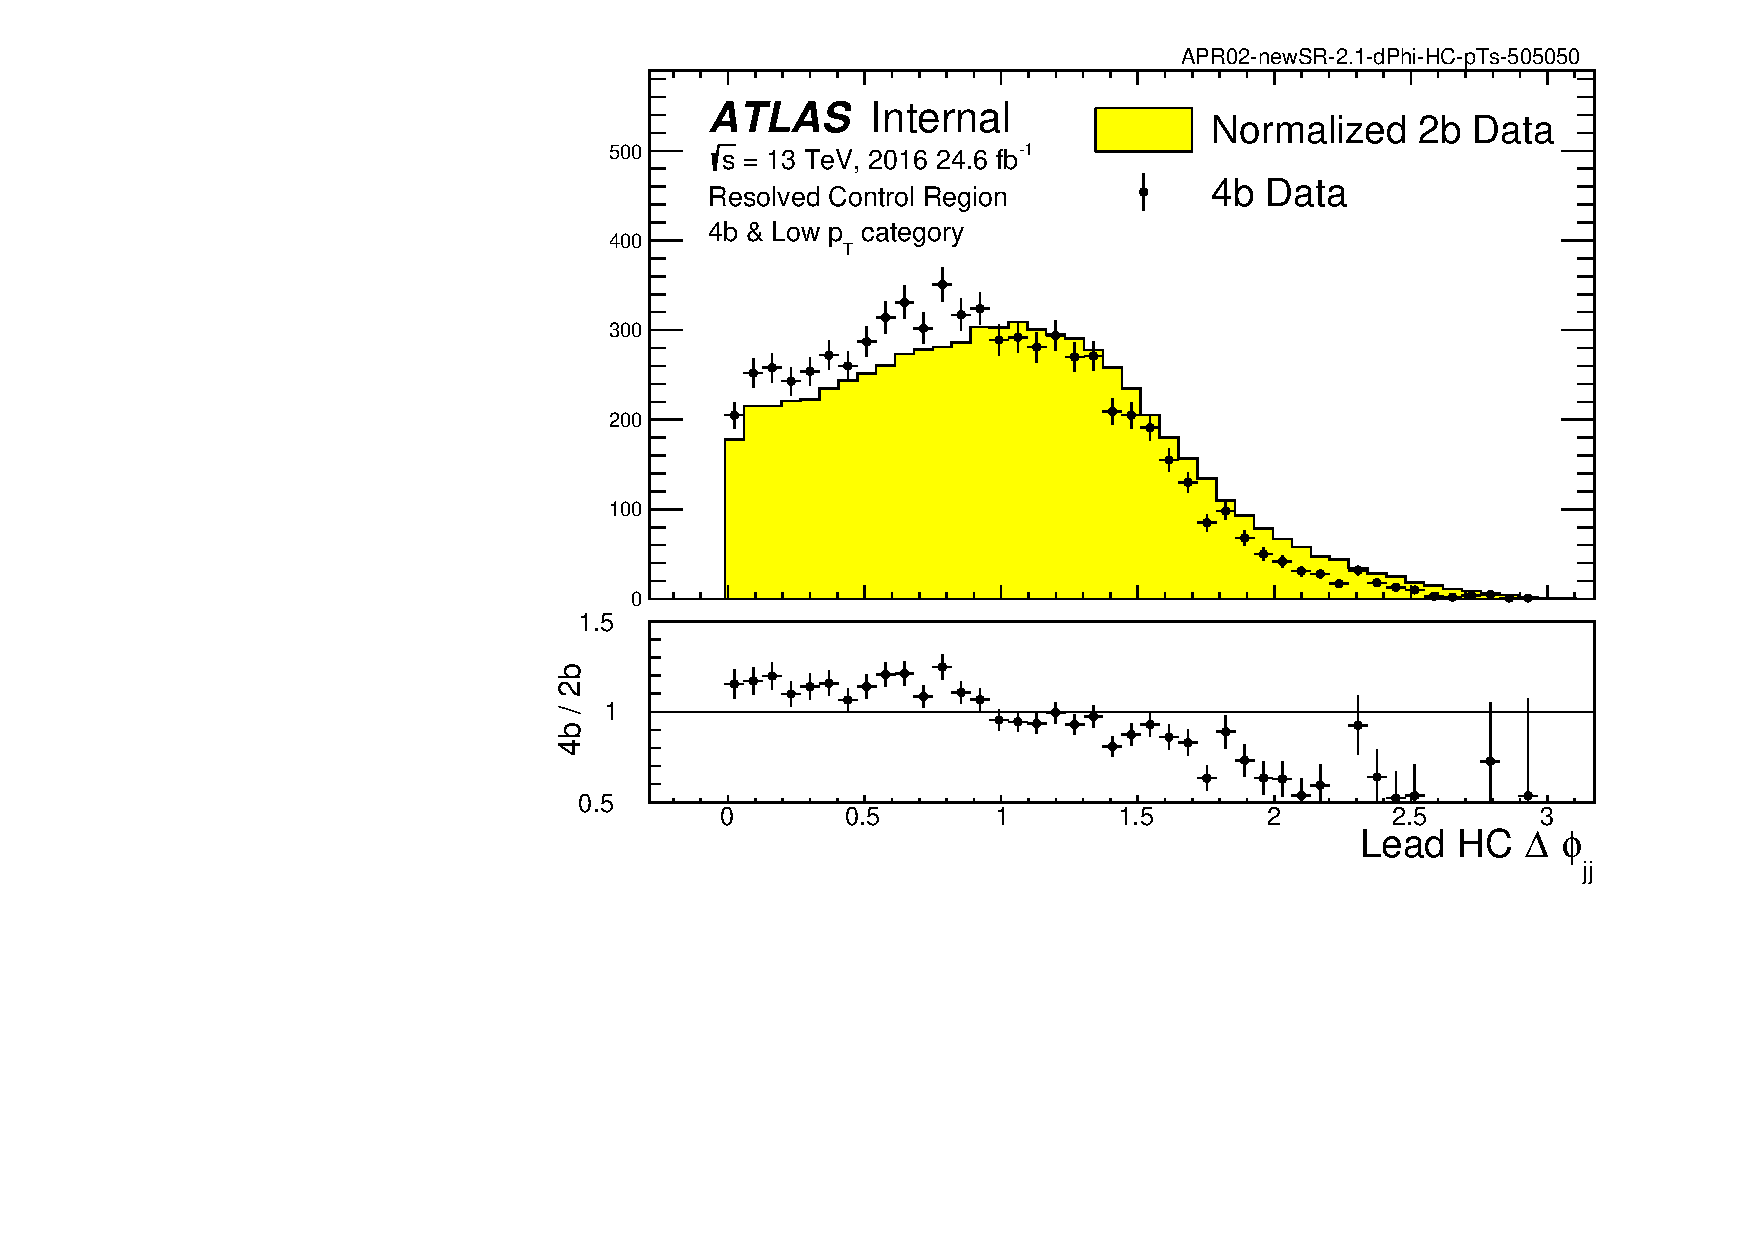
\includegraphics[width=0.4\textwidth]{\figpath{bkgdest-strategy/2016/bkgdest-dPhi-h1-norw-bstrap-med-shapesyst-Control-4bLowPtcat-NN-16.pdf}}
    }
    \subfloat{\label{fig:bkgdest16-dPhi-h1-Control-4bLowPtcat}%
            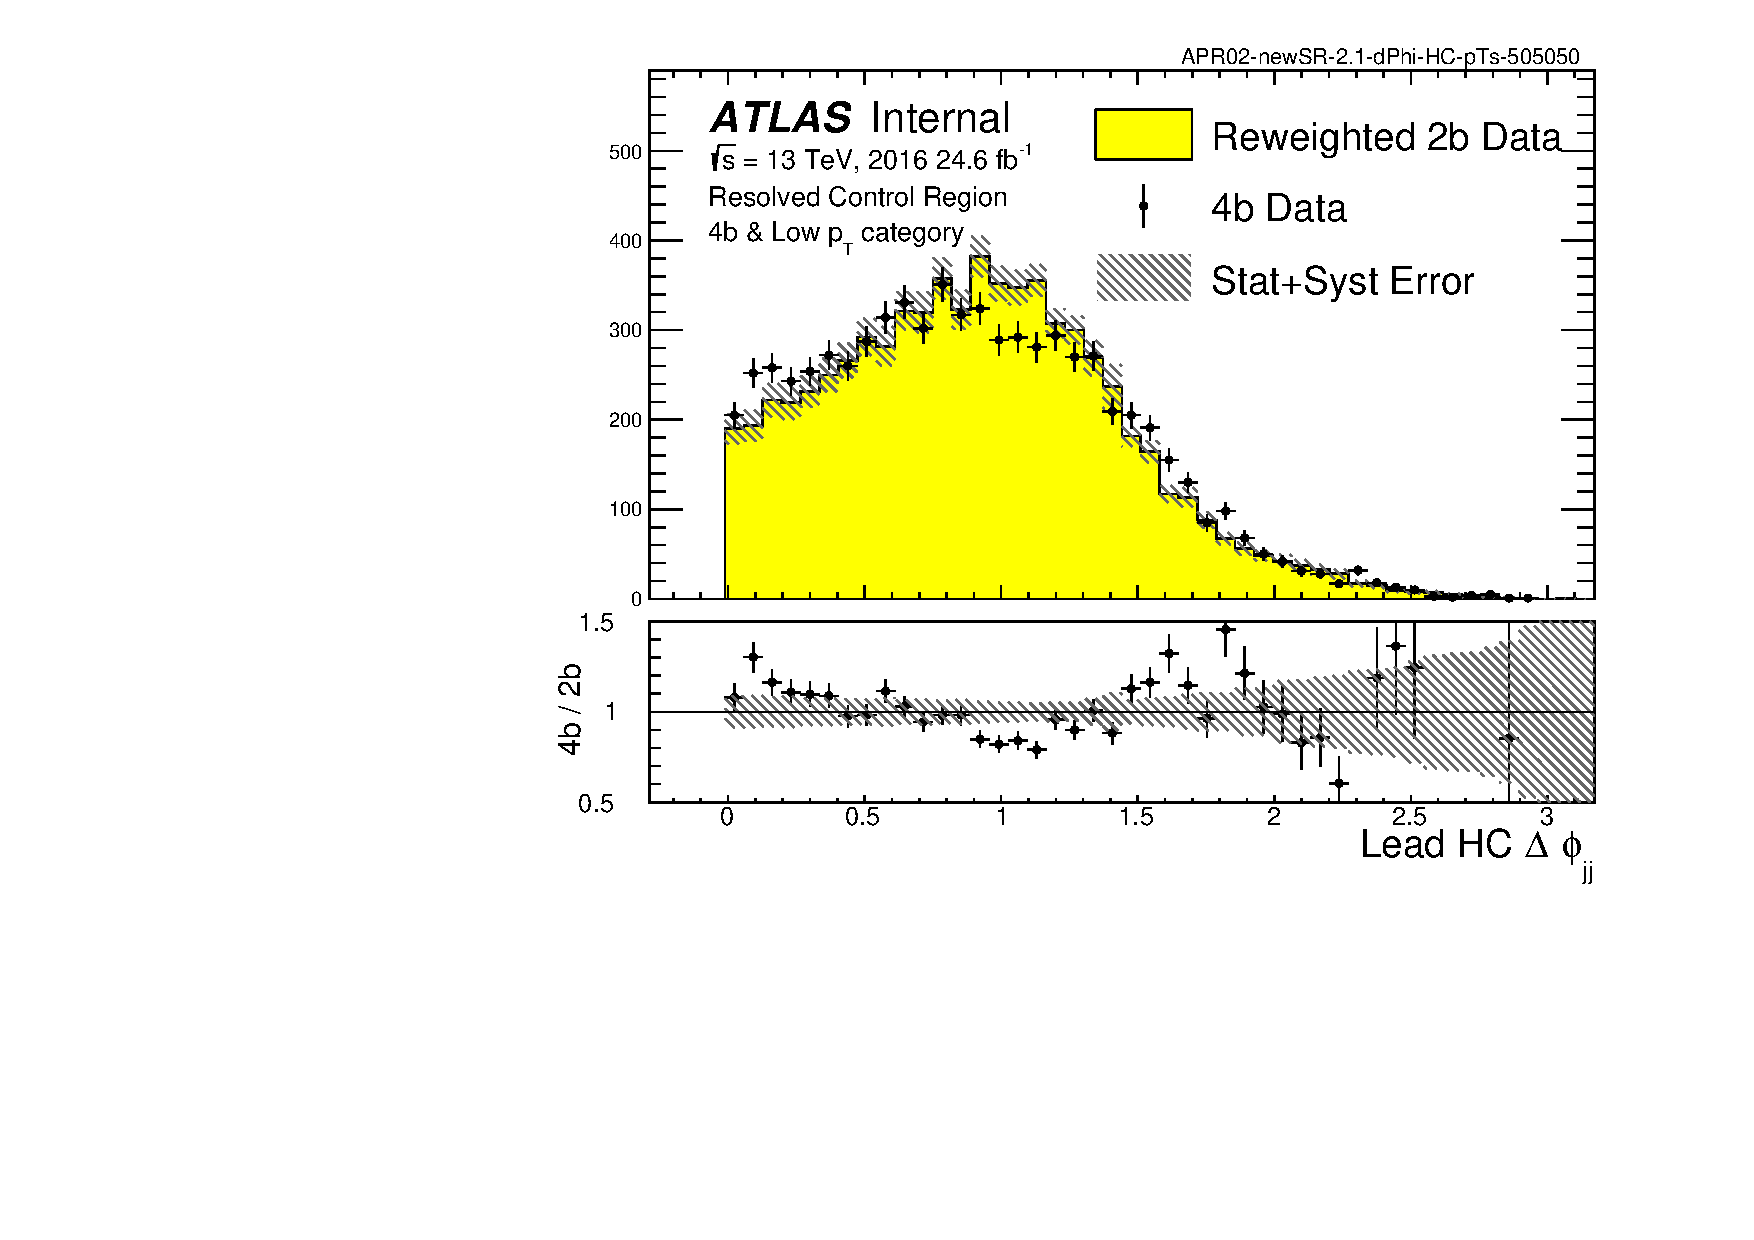
\includegraphics[width=0.4\textwidth]{\figpath{bkgdest-strategy/2016/bkgdest-dPhi-h1-bstrap-med-shapesyst-Control-4bLowPtcat-NN-16.pdf}}
    }

    \subfloat{\label{fig:bkgdest16-dPhi-h2-norw-Control-4bLowPtcat}%
            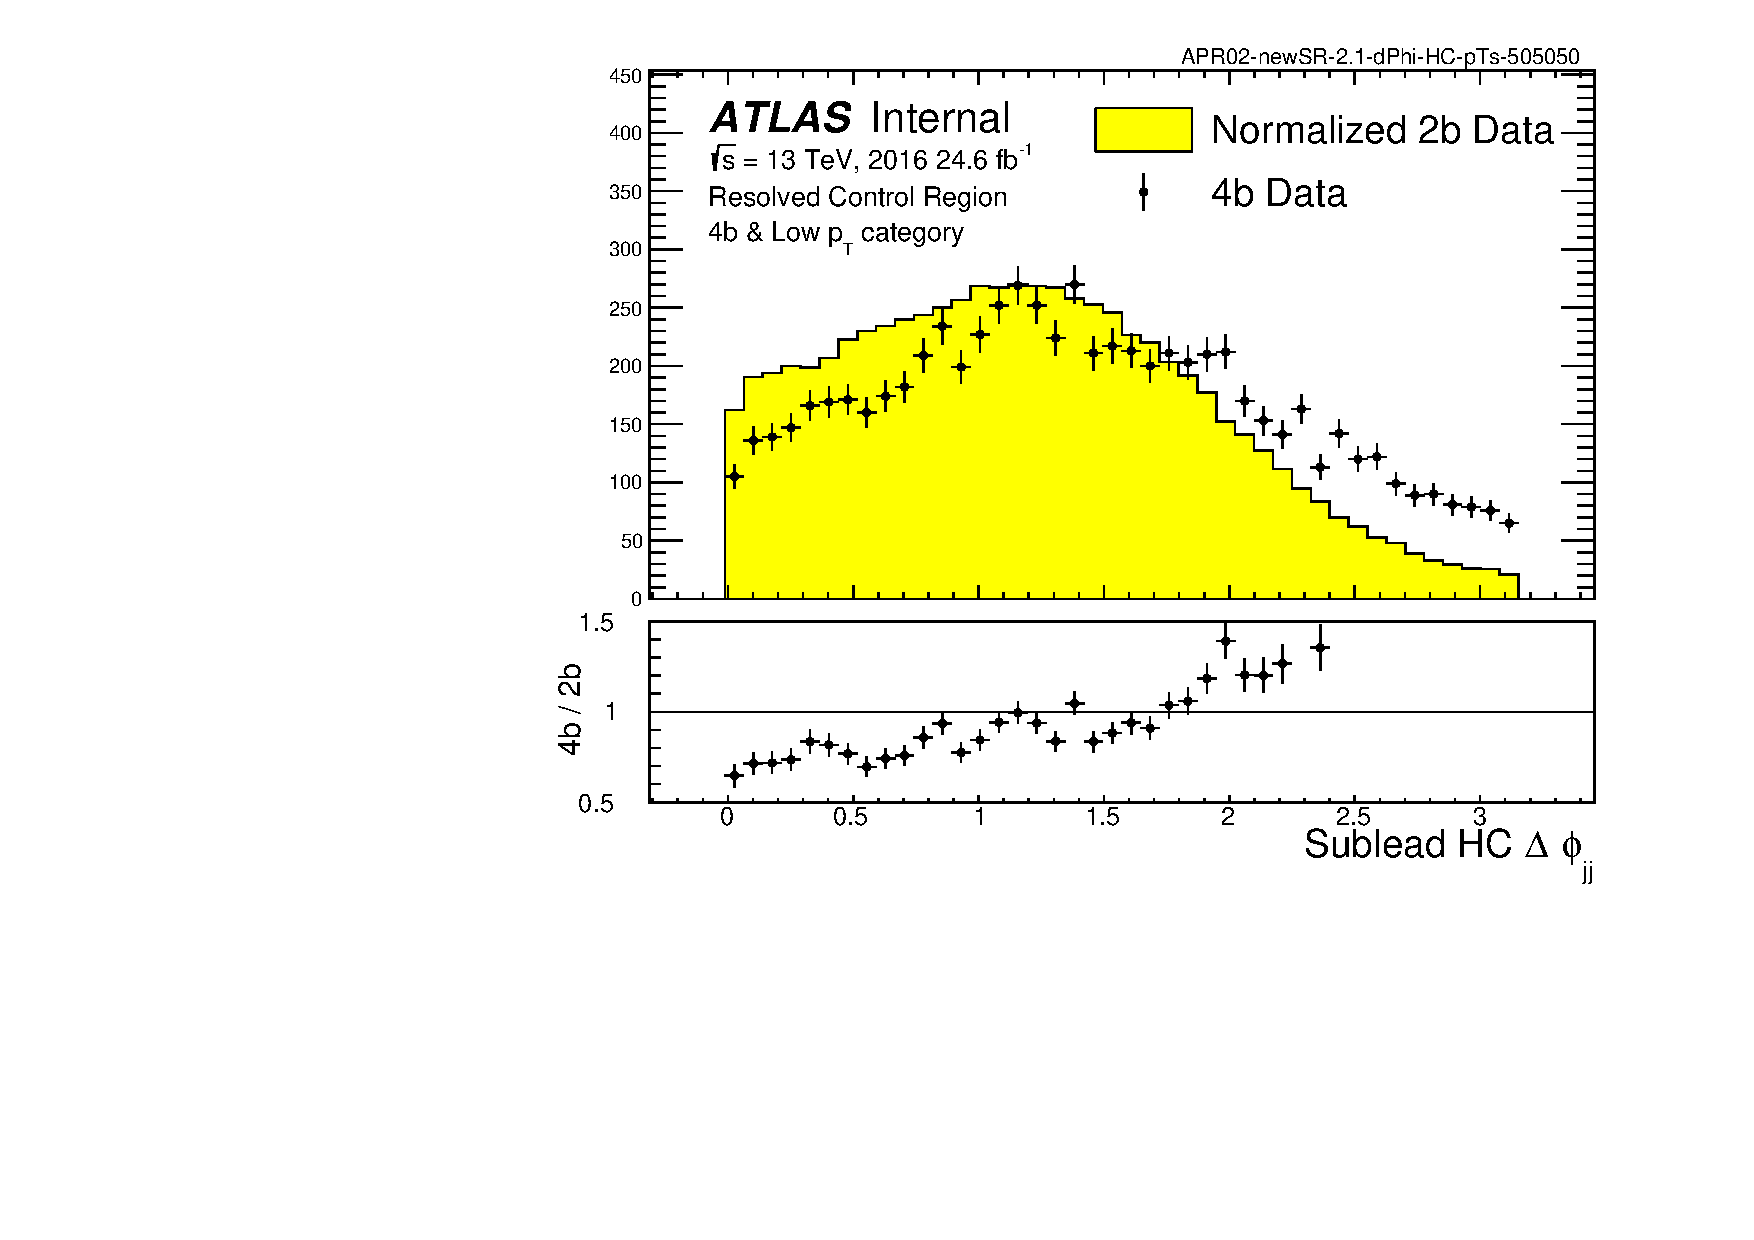
\includegraphics[width=0.4\textwidth]{\figpath{bkgdest-strategy/2016/bkgdest-dPhi-h2-norw-bstrap-med-shapesyst-Control-4bLowPtcat-NN-16.pdf}}
    }
    \subfloat{\label{fig:bkgdest16-dPhi-h2-Control-4bLowPtcat}%
            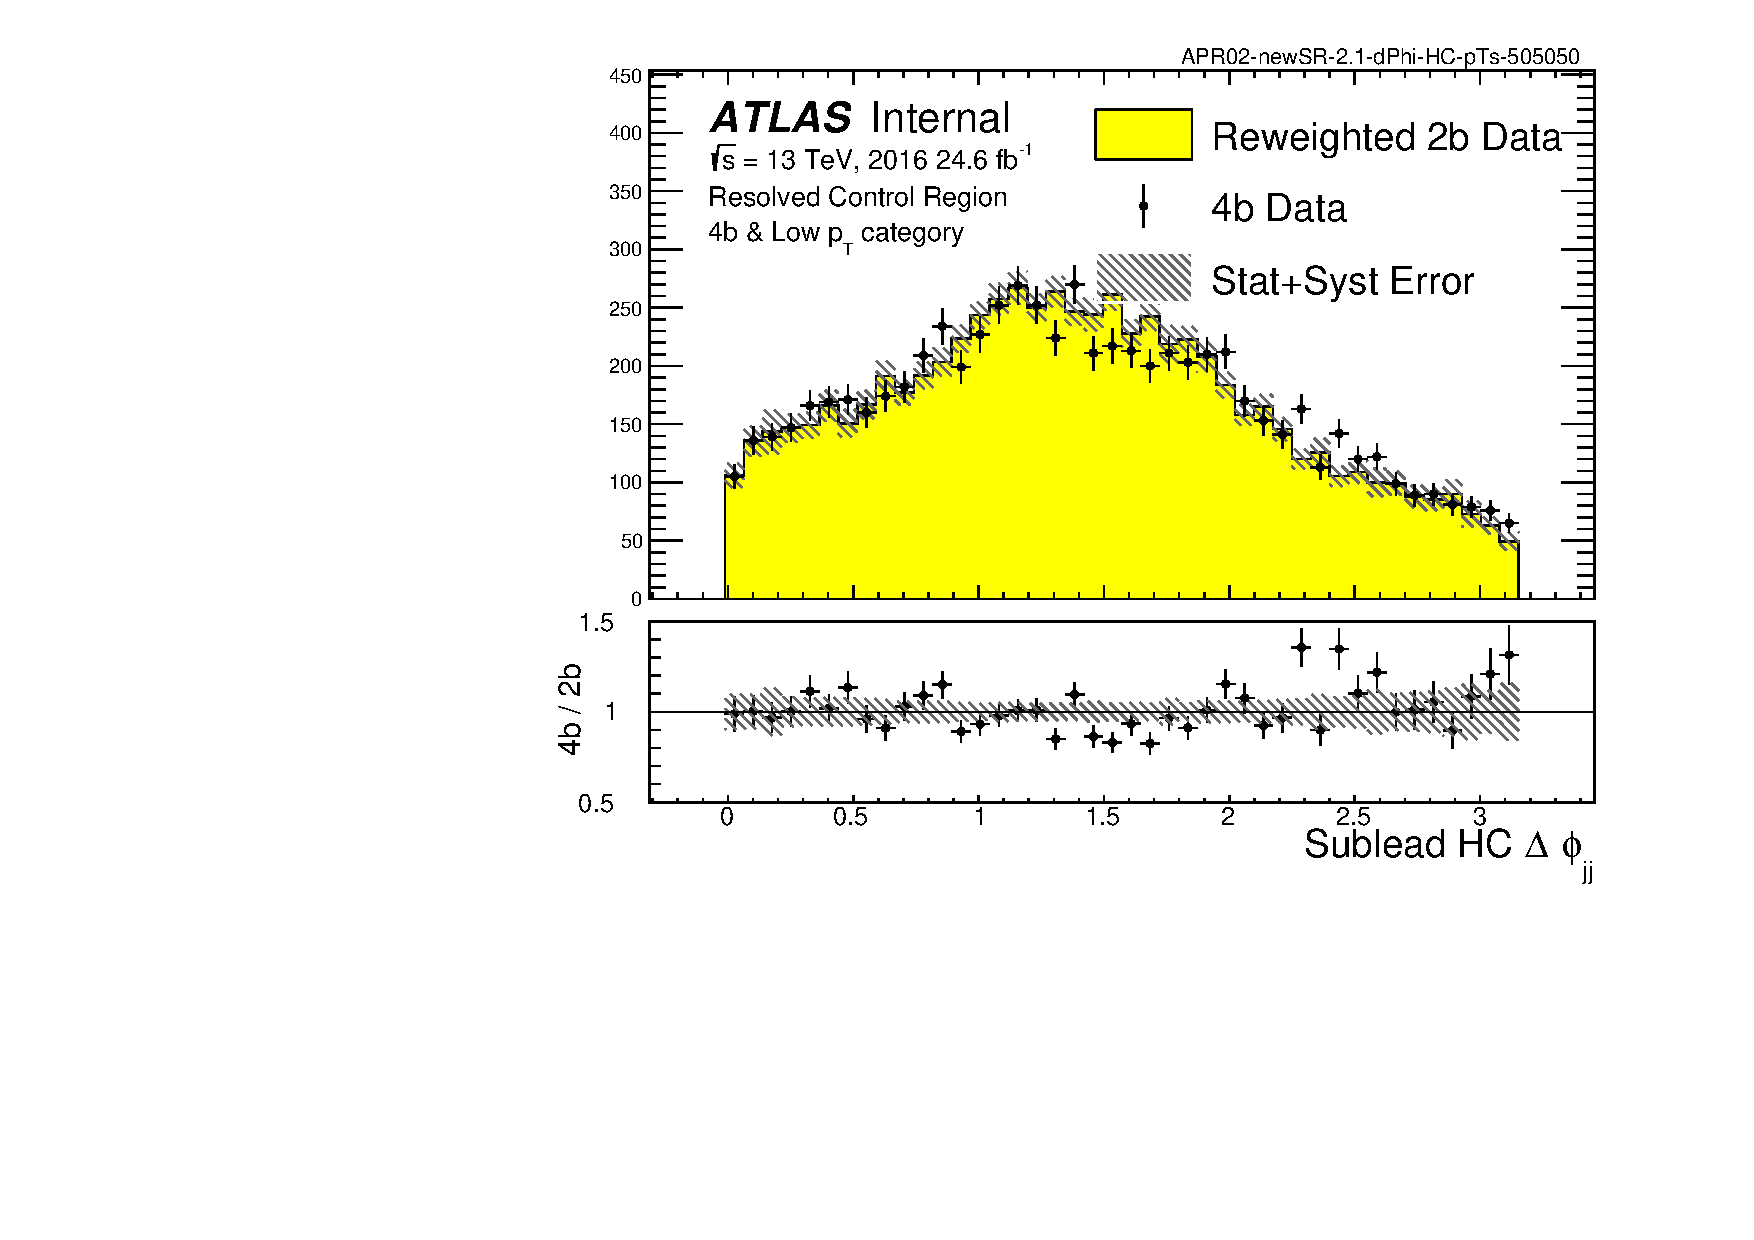
\includegraphics[width=0.4\textwidth]{\figpath{bkgdest-strategy/2016/bkgdest-dPhi-h2-bstrap-med-shapesyst-Control-4bLowPtcat-NN-16.pdf}}
    }

    \subfloat[Before reweighting]{\label{fig:bkgdest16-dR-hh-norw-Control-4bLowPtcat}%
            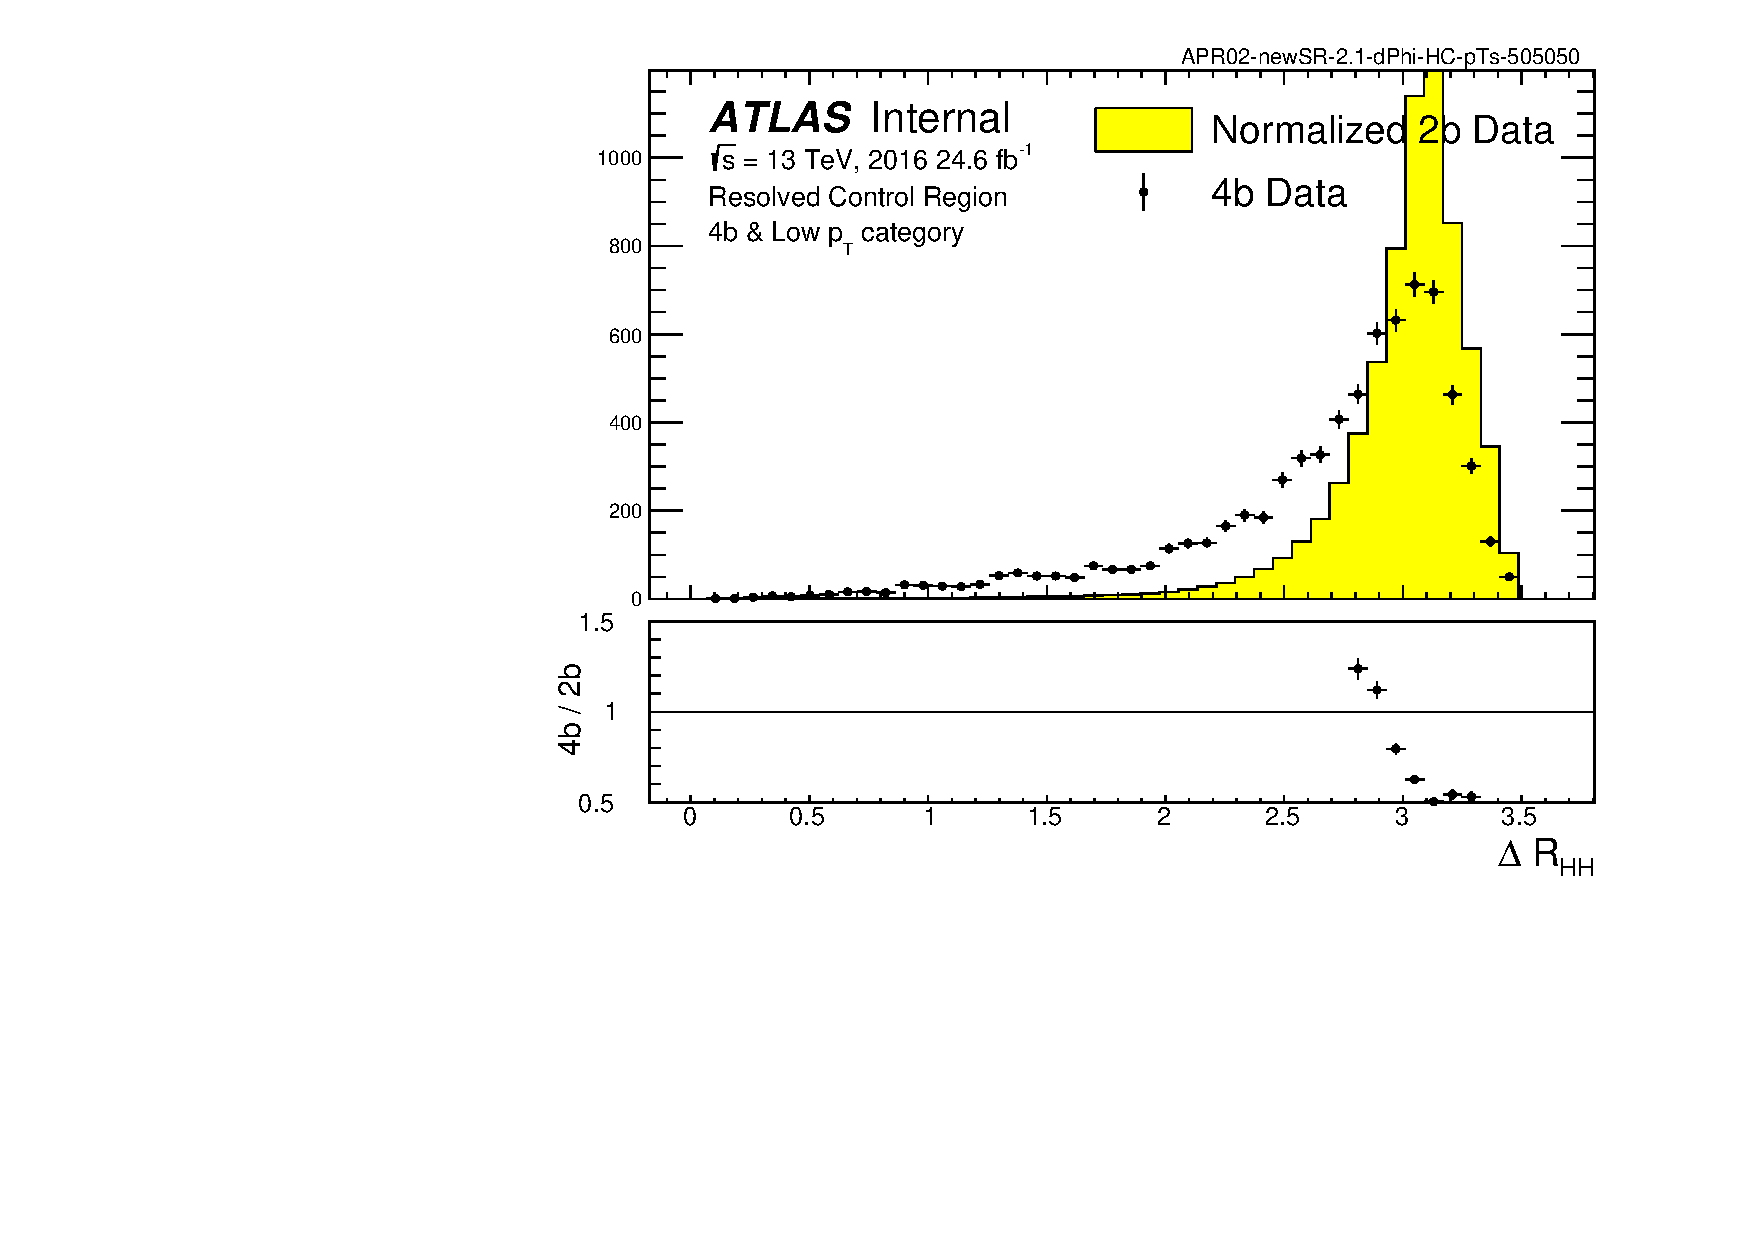
\includegraphics[width=0.4\textwidth]{\figpath{bkgdest-strategy/2016/bkgdest-dR-hh-norw-bstrap-med-shapesyst-Control-4bLowPtcat-NN-16.pdf}}
    }
    \subfloat[After reweighting]{\label{fig:bkgdest16-dR-hh-Control-4bLowPtcat}%
            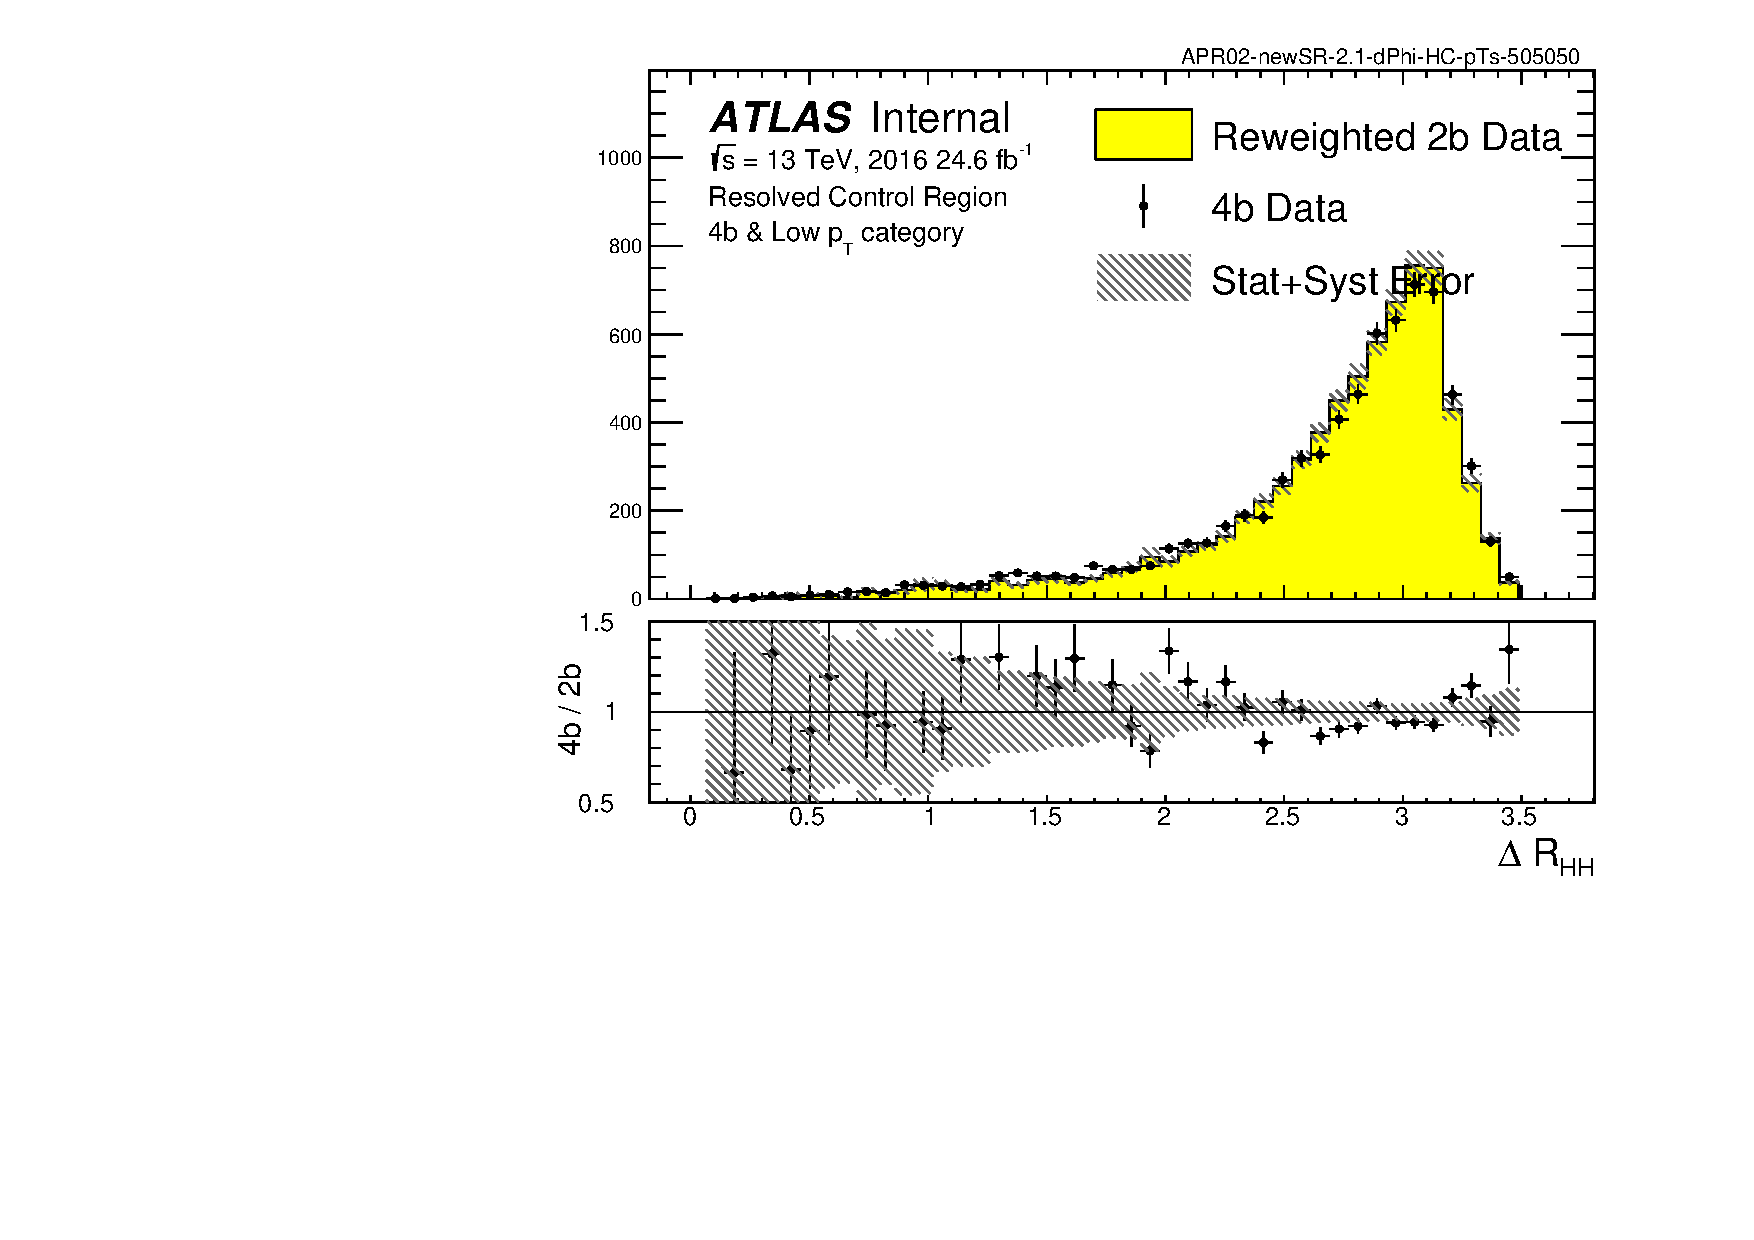
\includegraphics[width=0.4\textwidth]{\figpath{bkgdest-strategy/2016/bkgdest-dR-hh-bstrap-med-shapesyst-Control-4bLowPtcat-NN-16.pdf}}
    }
    \caption{Distributions of $\Delta\phi$-s between the jets in the leading and subleading Higgs candidates and \dr between the two Higgs candidates before and after reweighting, which includes log(pt)-s of the 1st and 3rd Higgs candidate jets, in the 2016 Control Region.}
    \label{fig:bkgdest16-3-Control-4bLowPtcat}
\end{figure}


\begin{figure}[ht]
    \centering
    \subfloat{\label{fig:bkgdest16-pt-hh-norw-Control-4bLowPtcat}%
            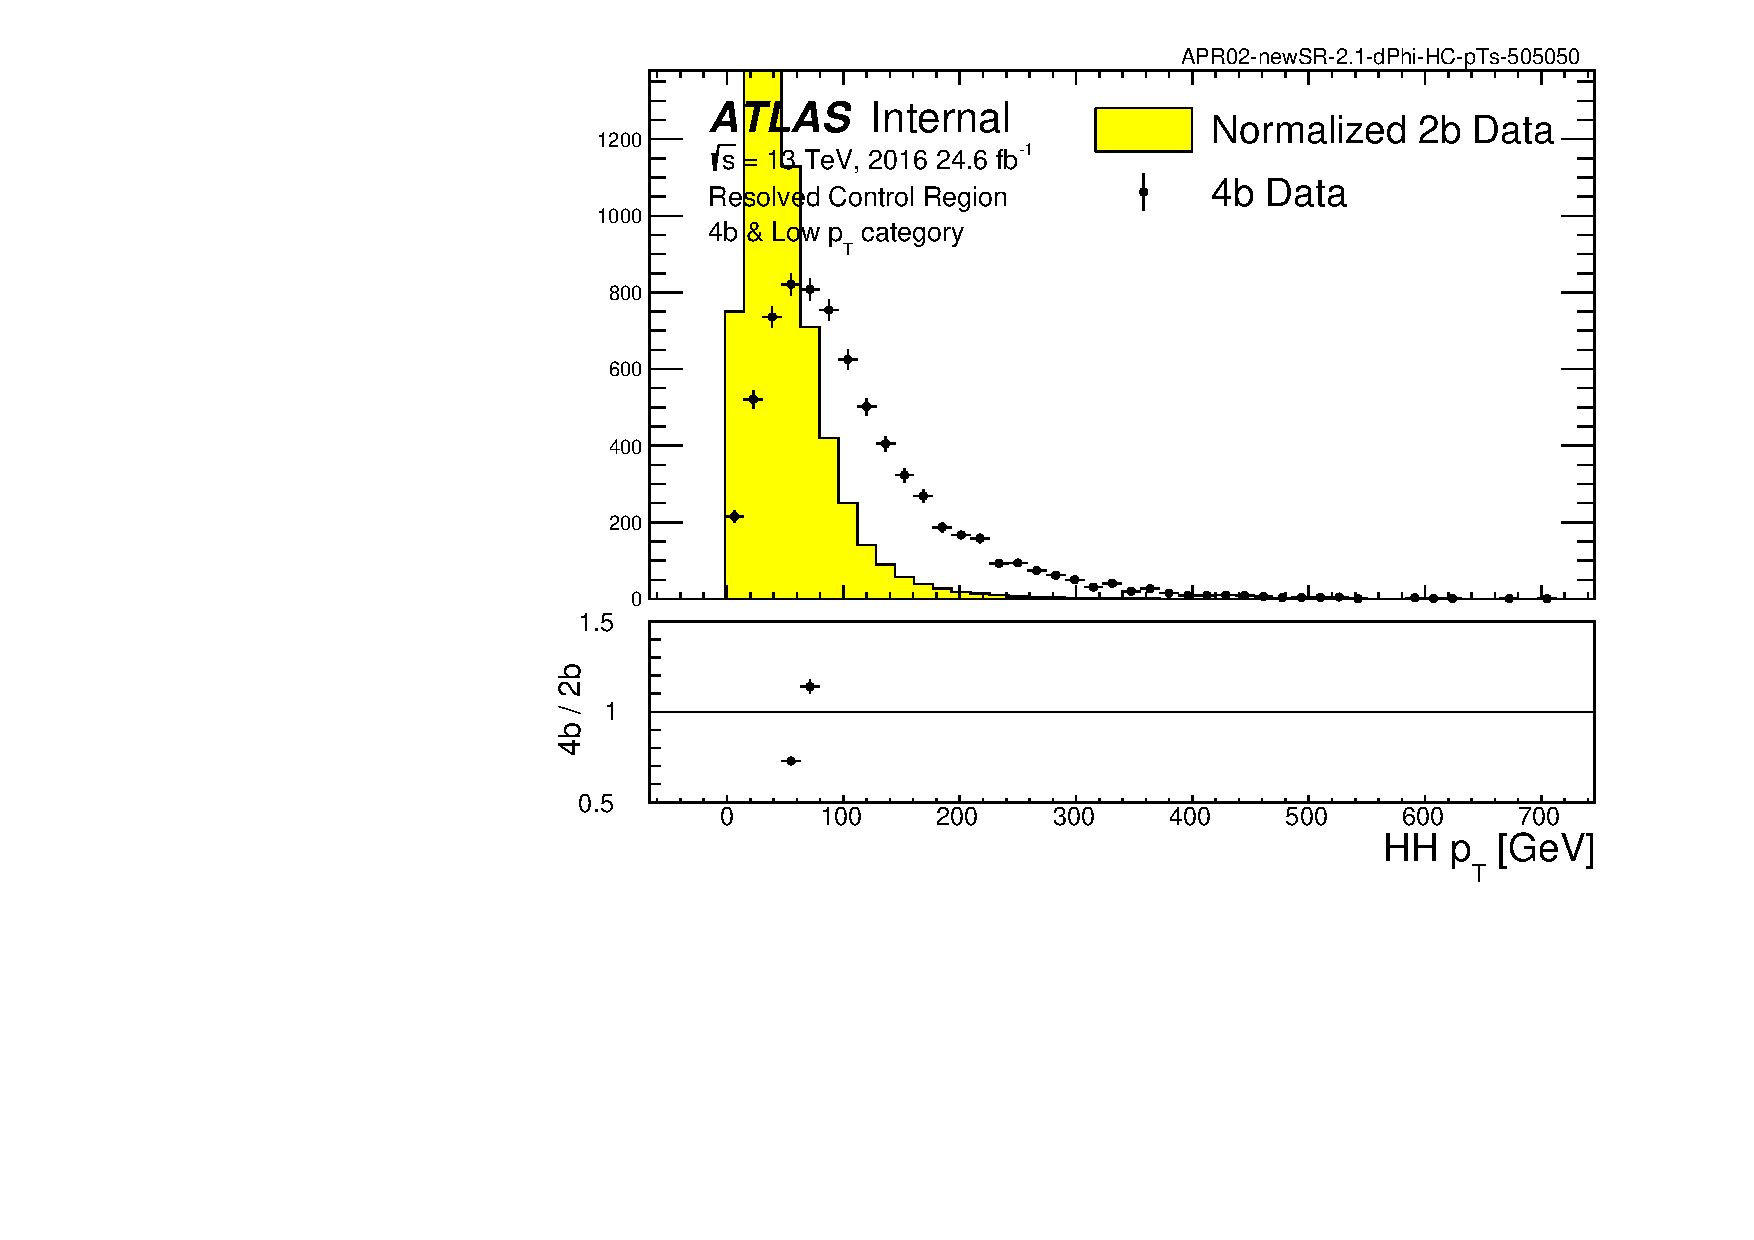
\includegraphics[width=0.4\textwidth]{\figpath{bkgdest-strategy/2016/bkgdest-pt-hh-norw-bstrap-med-shapesyst-Control-4bLowPtcat-NN-16.pdf}}
    }
    \subfloat{\label{fig:bkgdest16-pt-hh-Control-4bLowPtcat}%
            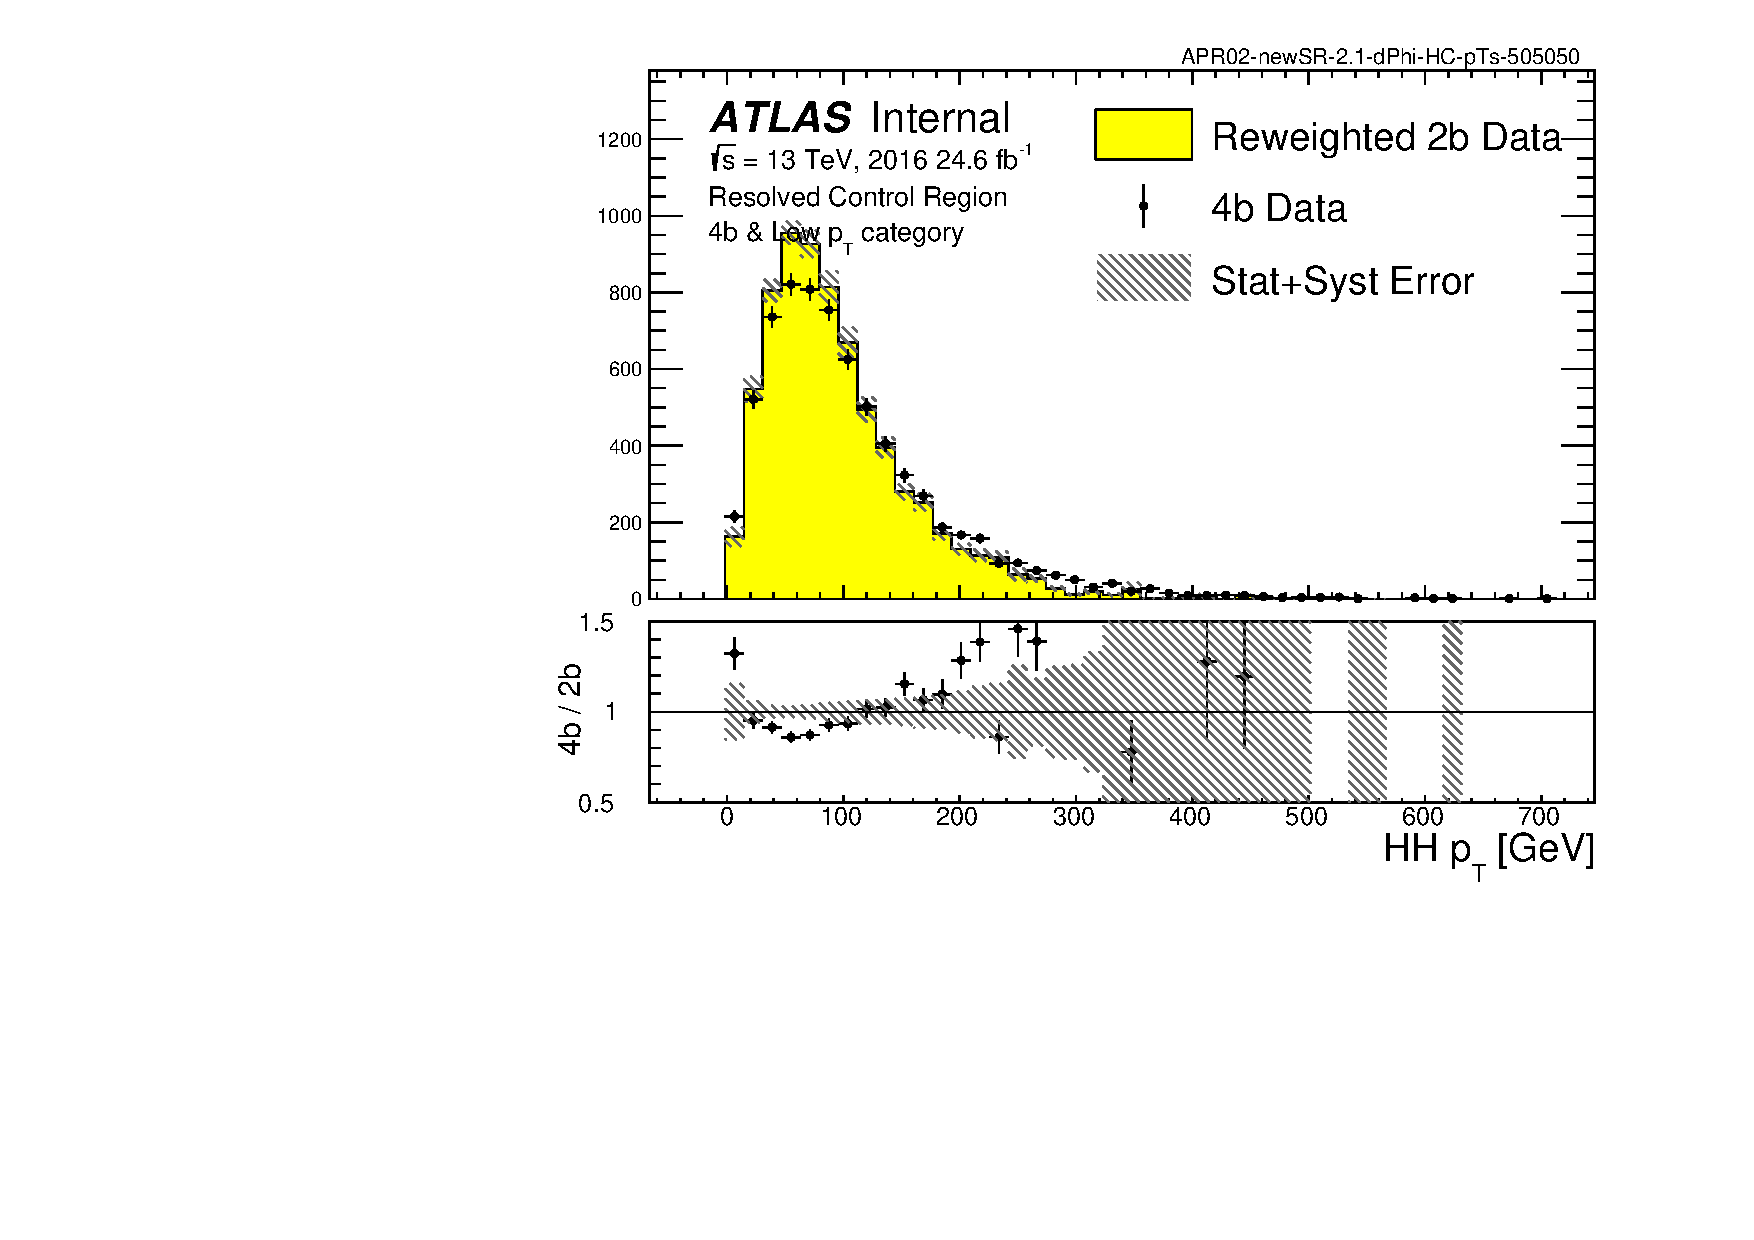
\includegraphics[width=0.4\textwidth]{\figpath{bkgdest-strategy/2016/bkgdest-pt-hh-bstrap-med-shapesyst-Control-4bLowPtcat-NN-16.pdf}}
    }
 
    \subfloat{\label{fig:bkgdest16-X-wt-tag-norw-Control-4bLowPtcat}%
            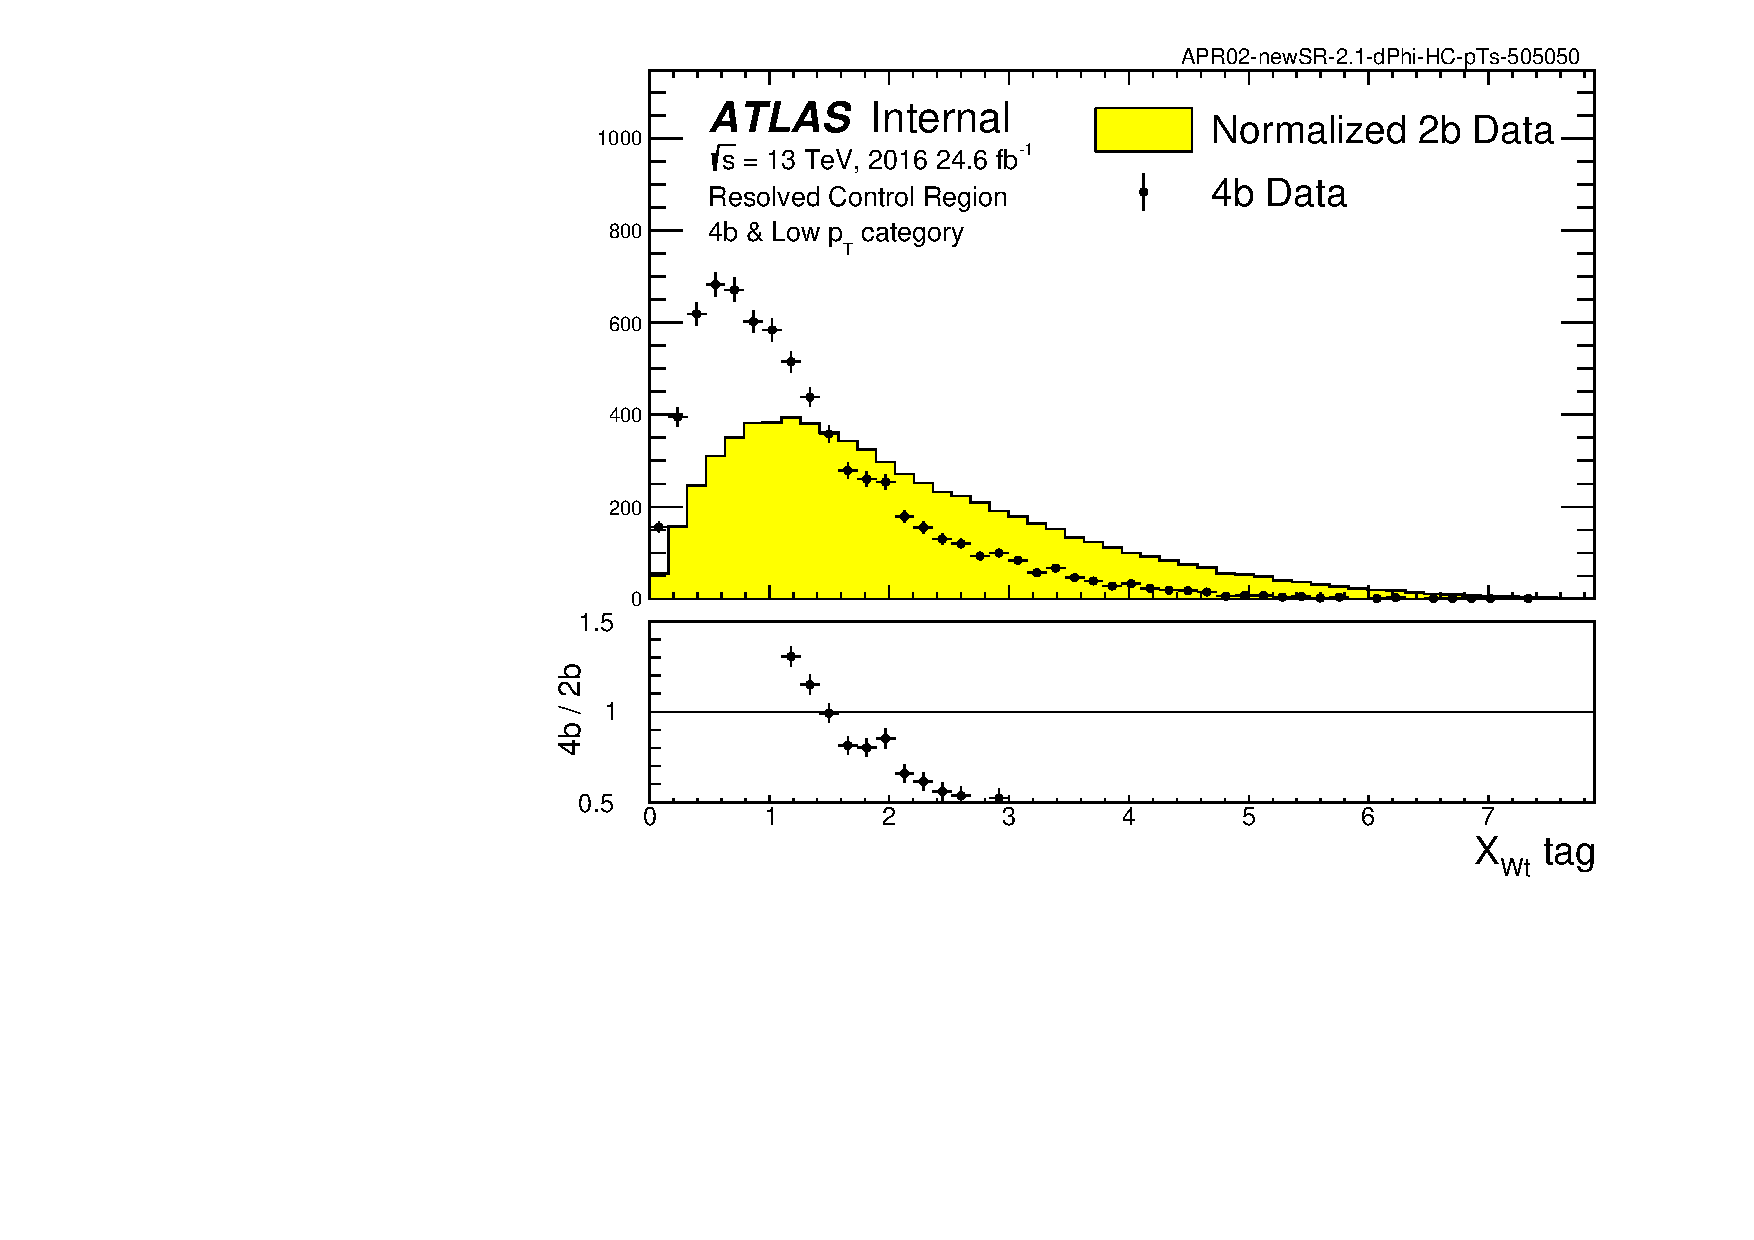
\includegraphics[width=0.4\textwidth]{\figpath{bkgdest-strategy/2016/bkgdest-X-wt-tag-norw-bstrap-med-shapesyst-Control-4bLowPtcat-NN-16.pdf}}
    }
    \subfloat{\label{fig:bkgdest16-X-wt-tag-Control-4bLowPtcat}%
            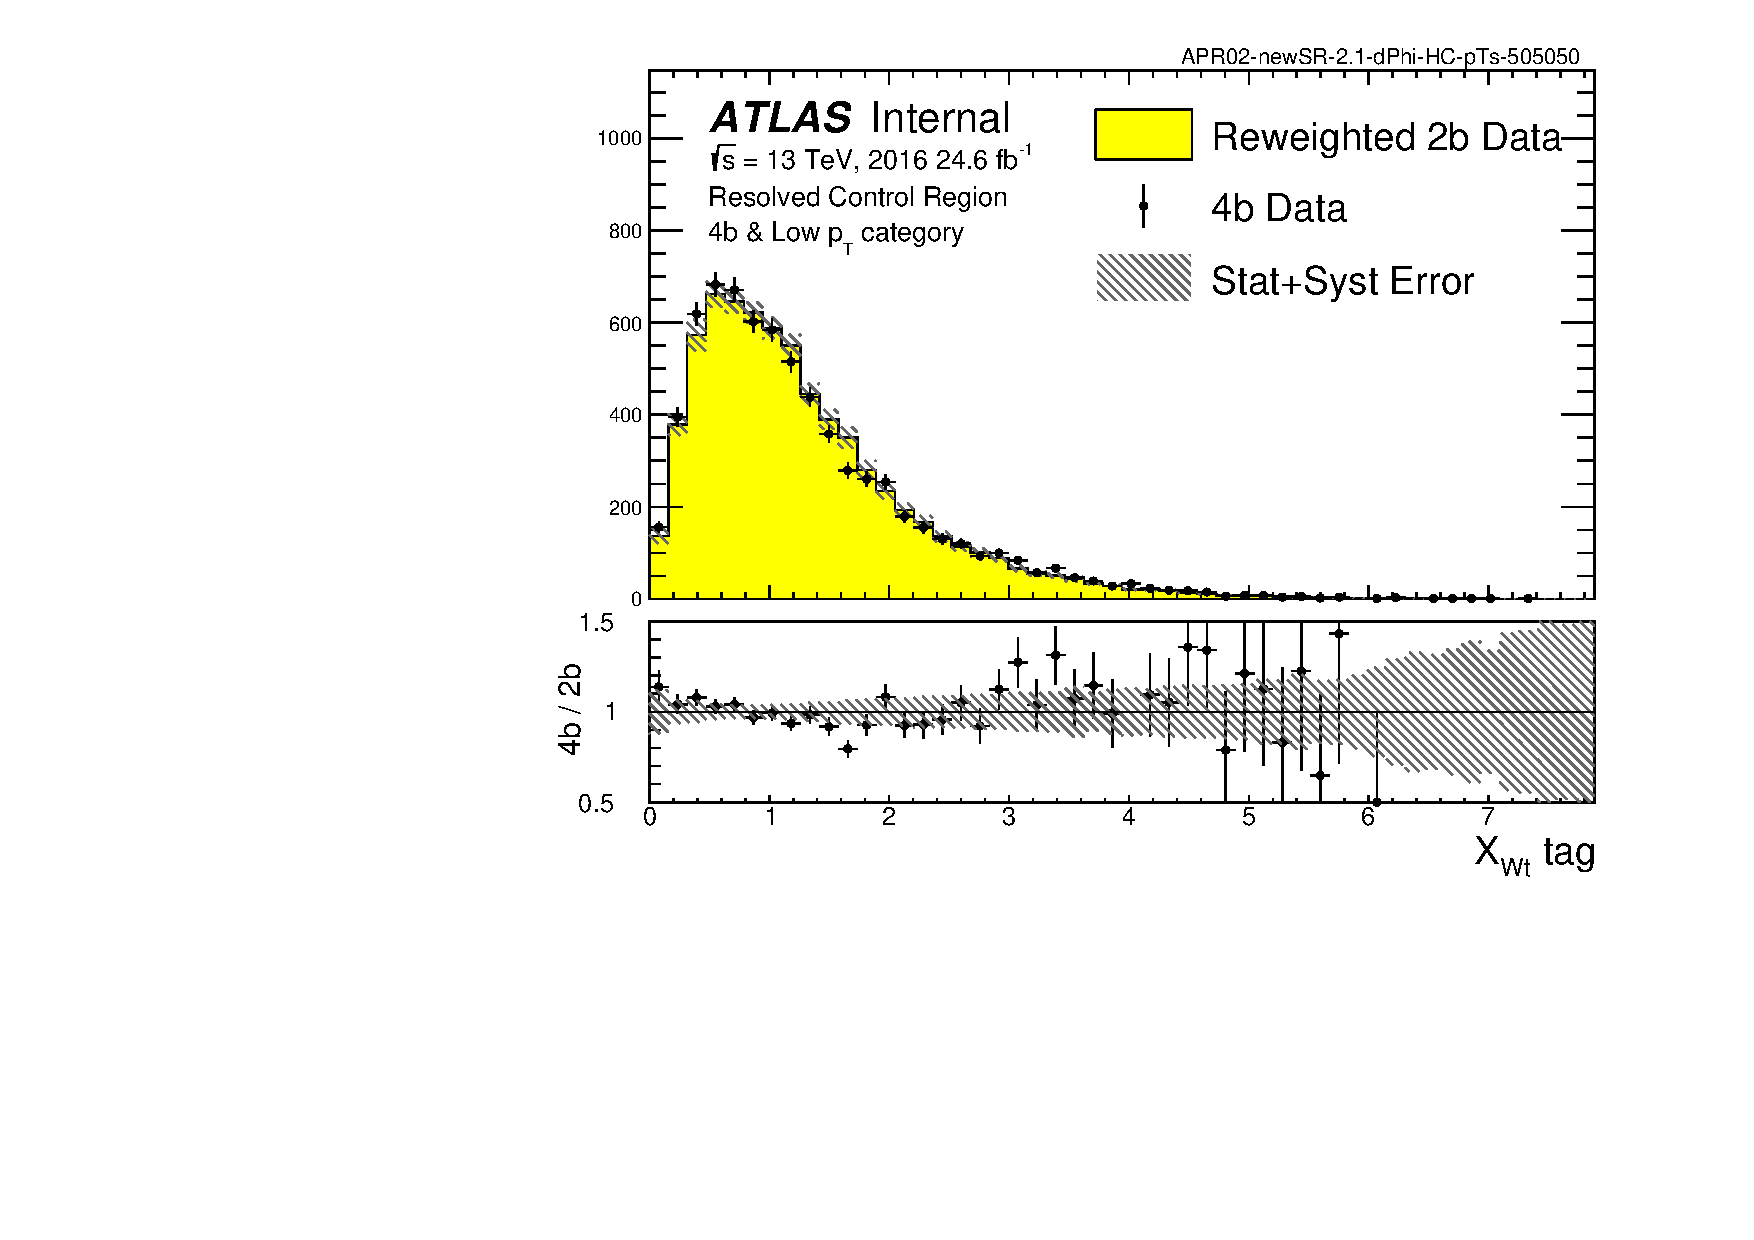
\includegraphics[width=0.4\textwidth]{\figpath{bkgdest-strategy/2016/bkgdest-X-wt-tag-bstrap-med-shapesyst-Control-4bLowPtcat-NN-16.pdf}}
    }

    \subfloat[Before reweighting]{\label{fig:bkgdest16-njets-norw-Control-4bLowPtcat}%
            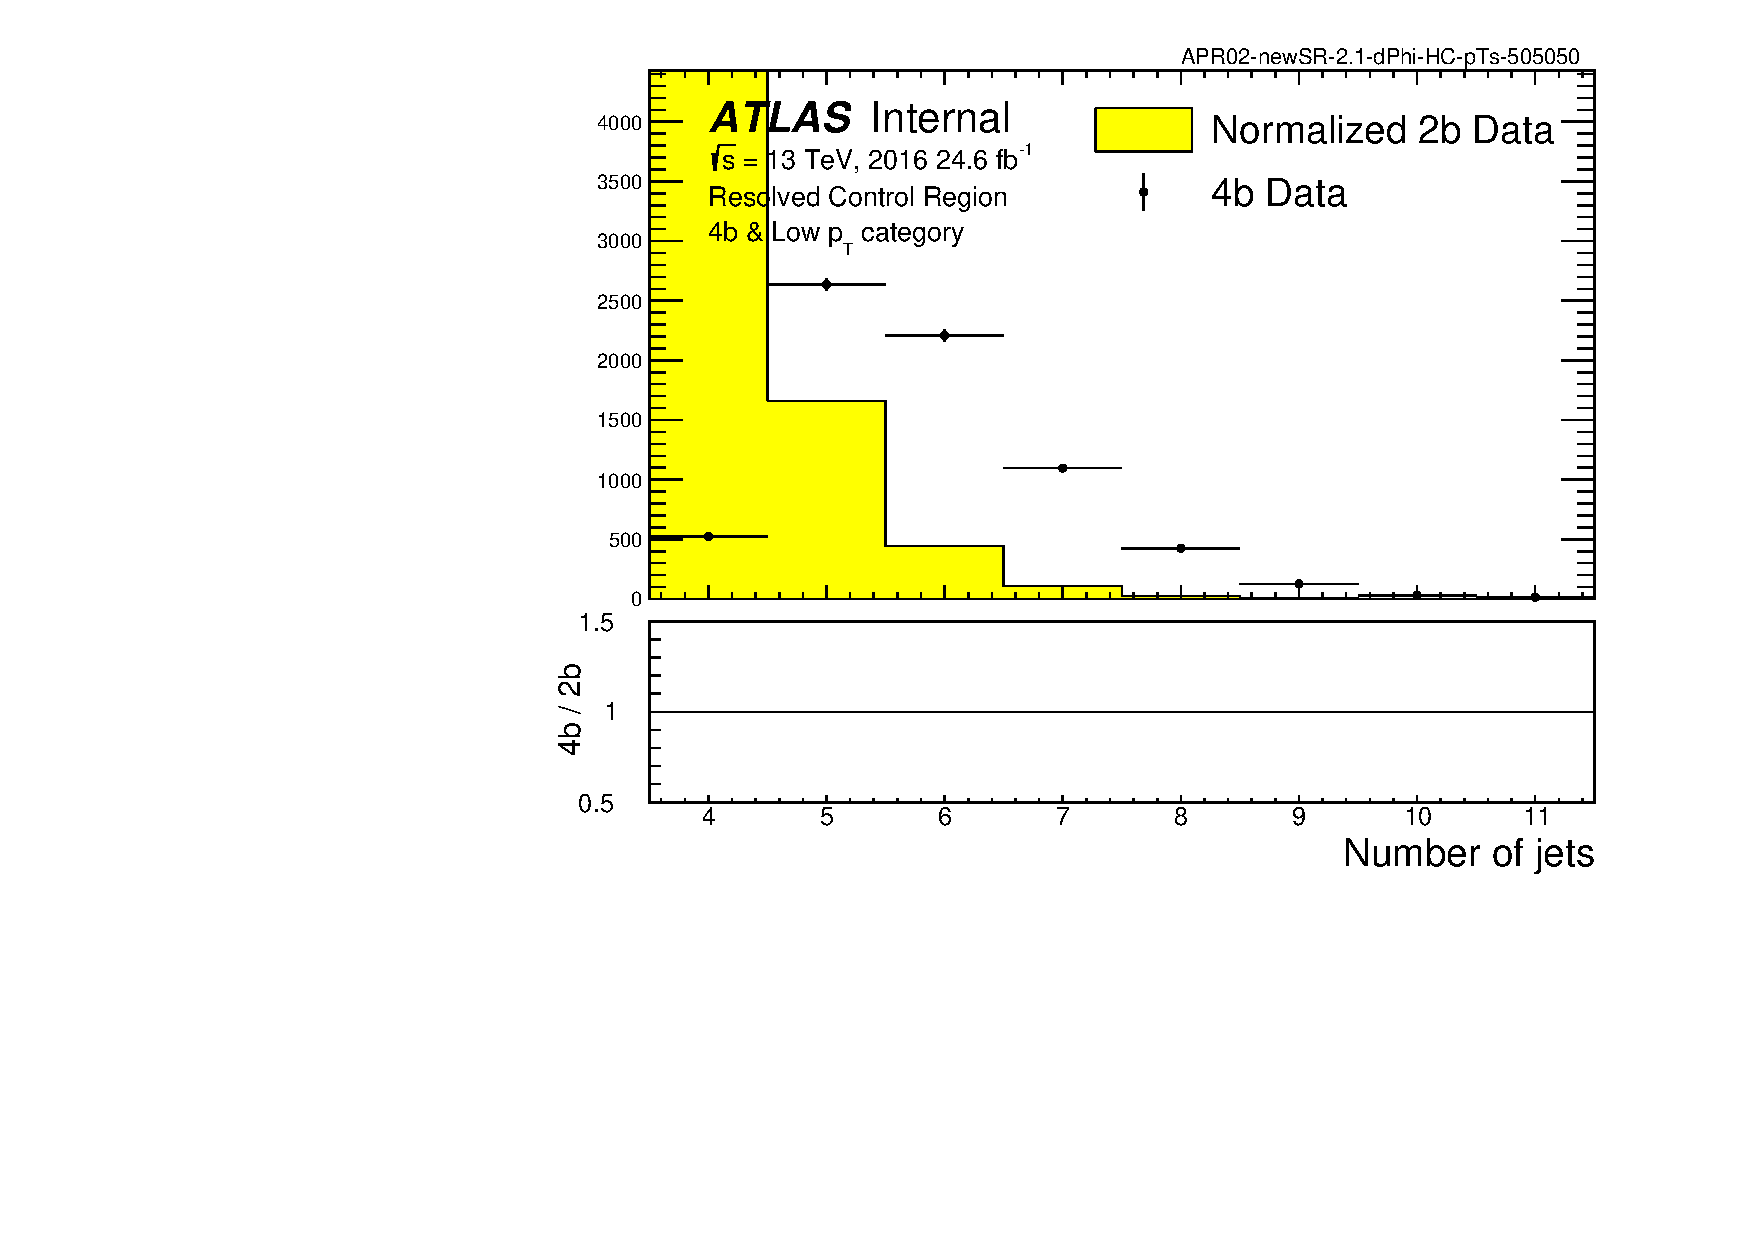
\includegraphics[width=0.4\textwidth]{\figpath{bkgdest-strategy/2016/bkgdest-njets-norw-bstrap-med-shapesyst-Control-4bLowPtcat-NN-16.pdf}}
    }
    \subfloat[After reweighting]{\label{fig:bkgdest16-njets-Control-4bLowPtcat}%
            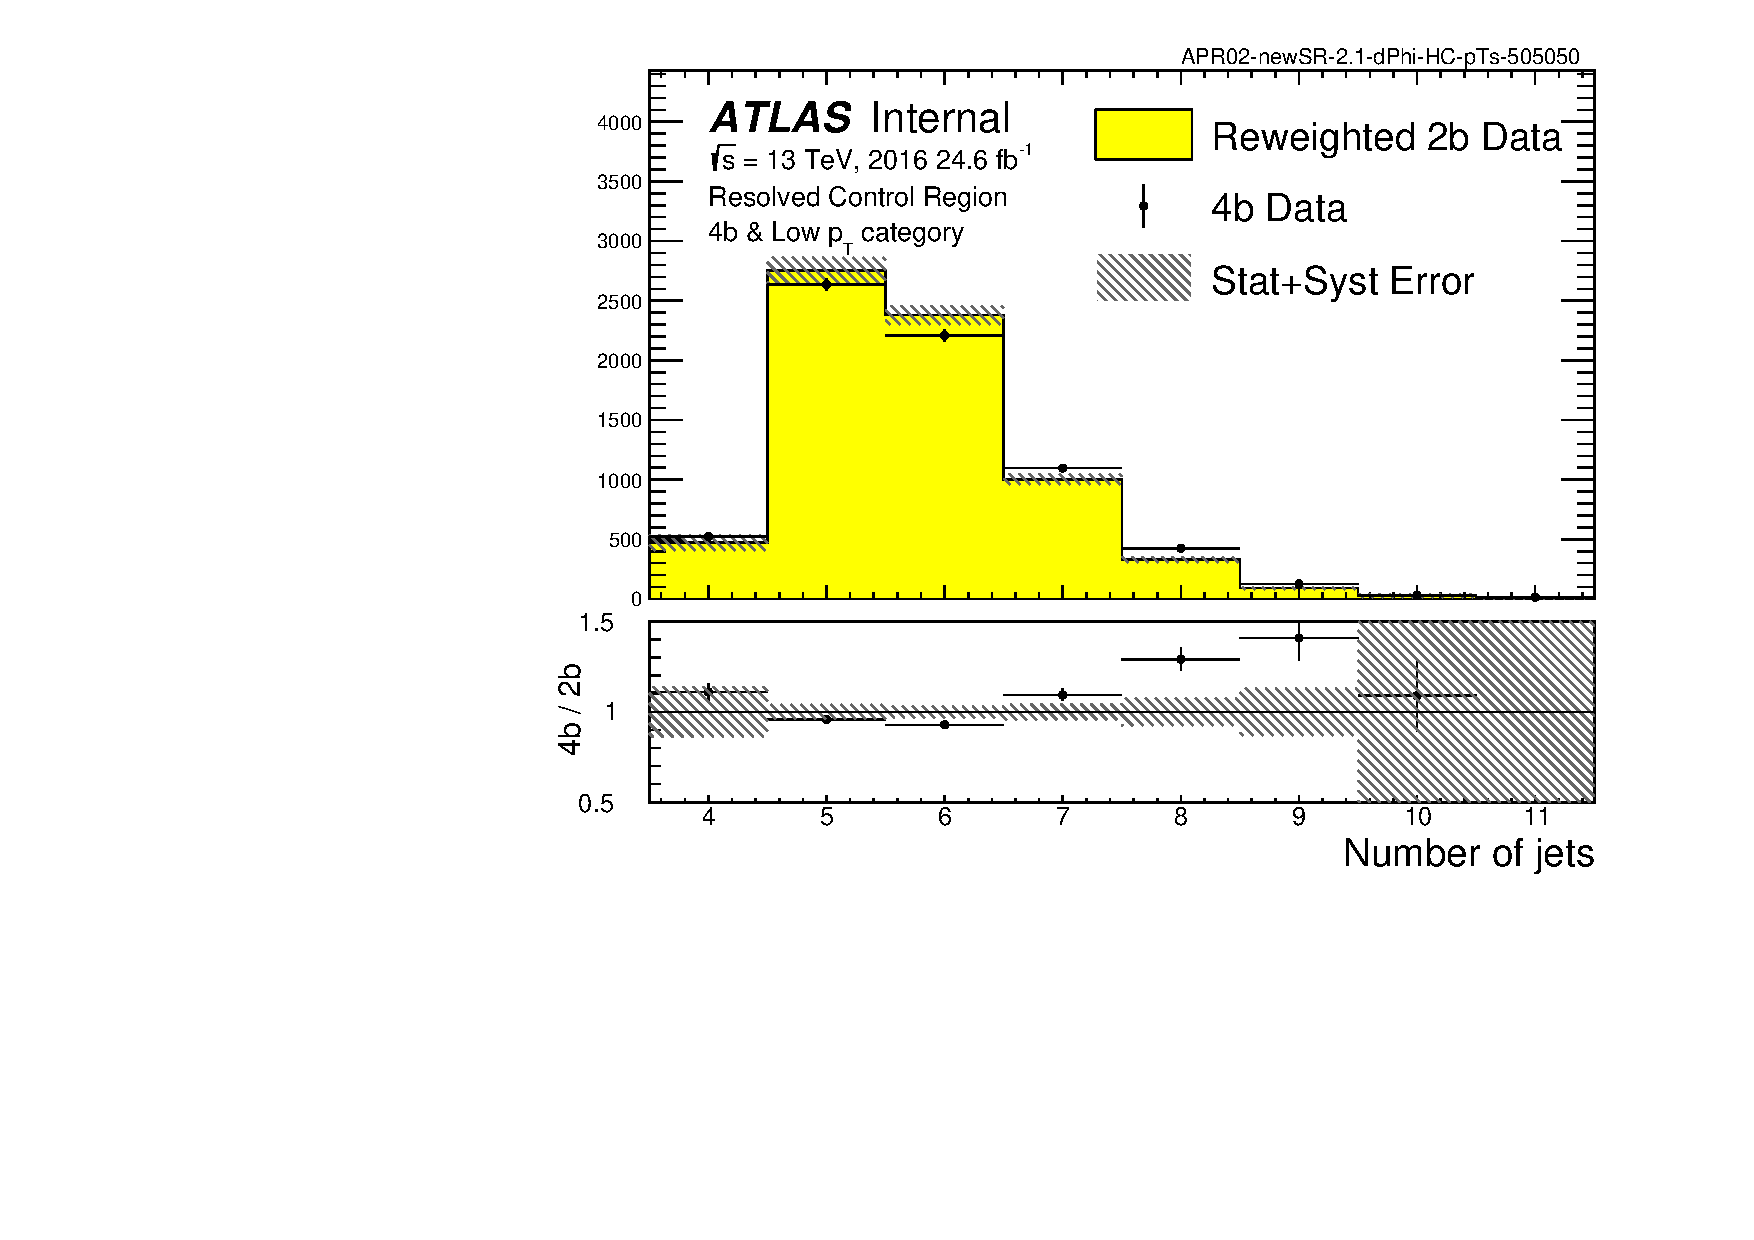
\includegraphics[width=0.4\textwidth]{\figpath{bkgdest-strategy/2016/bkgdest-njets-bstrap-med-shapesyst-Control-4bLowPtcat-NN-16.pdf}}
    }

    \caption{Distributions of log(\pt) of the di-higgs system, $X_{wt}$ used for the \ttbar veto and number of jets in the events before and after reweighting, which includes log(pt)-s of the 1st and 3rd Higgs candidate jets, in the 2016 Control Region.}
    \label{fig:bkgdest16-4-Control-4bLowPtcat}
\end{figure}


\begin{figure}[ht]
    \centering
    \subfloat[Before reweighting]{\label{fig:bkgdest16-m-hh-norw-Control-4bLowPtcat}%
            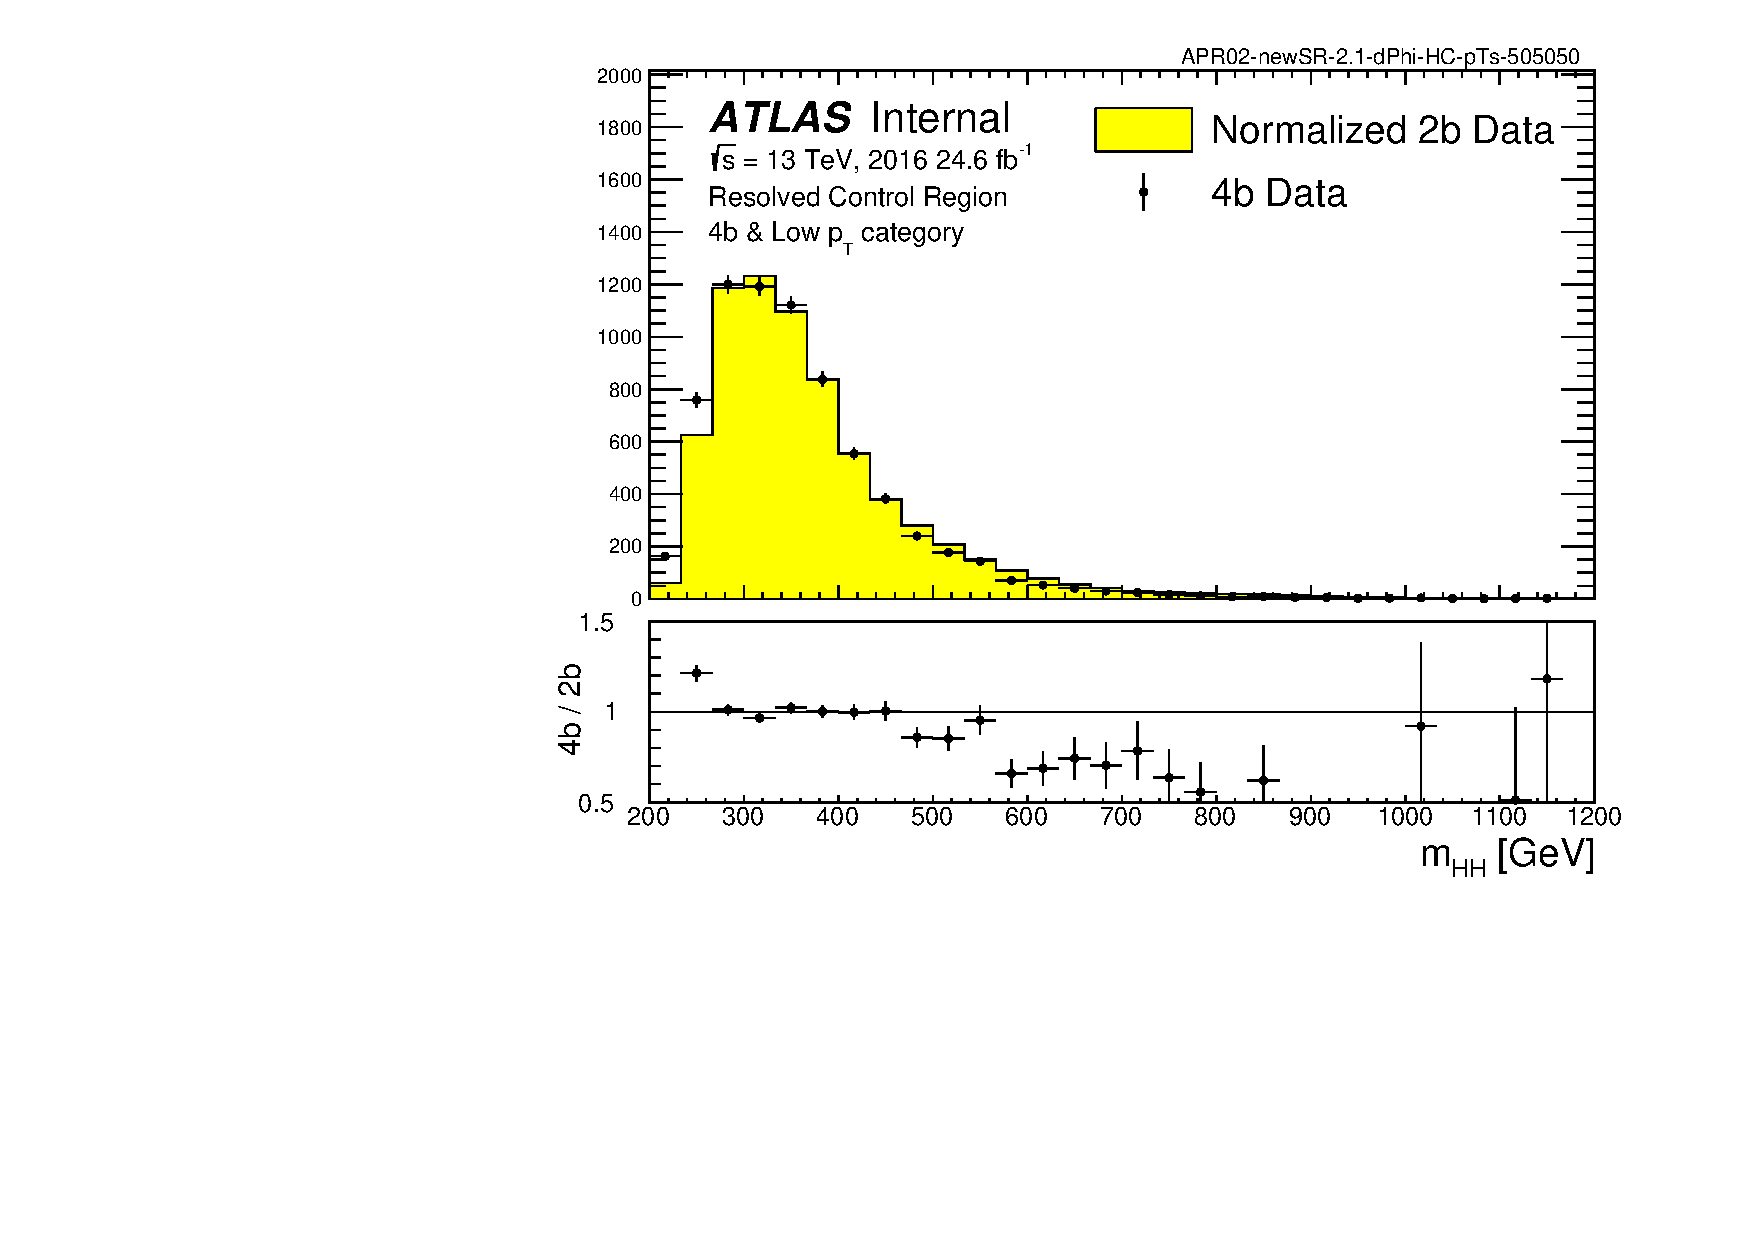
\includegraphics[width=0.4\textwidth]{\figpath{bkgdest-strategy/2016/bkgdest-m-hh-norw-bstrap-med-shapesyst-Control-4bLowPtcat-NN-16.pdf}}
    }
    \subfloat[After reweighting]{\label{fig:bkgdest16-m-hh-Control-4bLowPtcat}%
            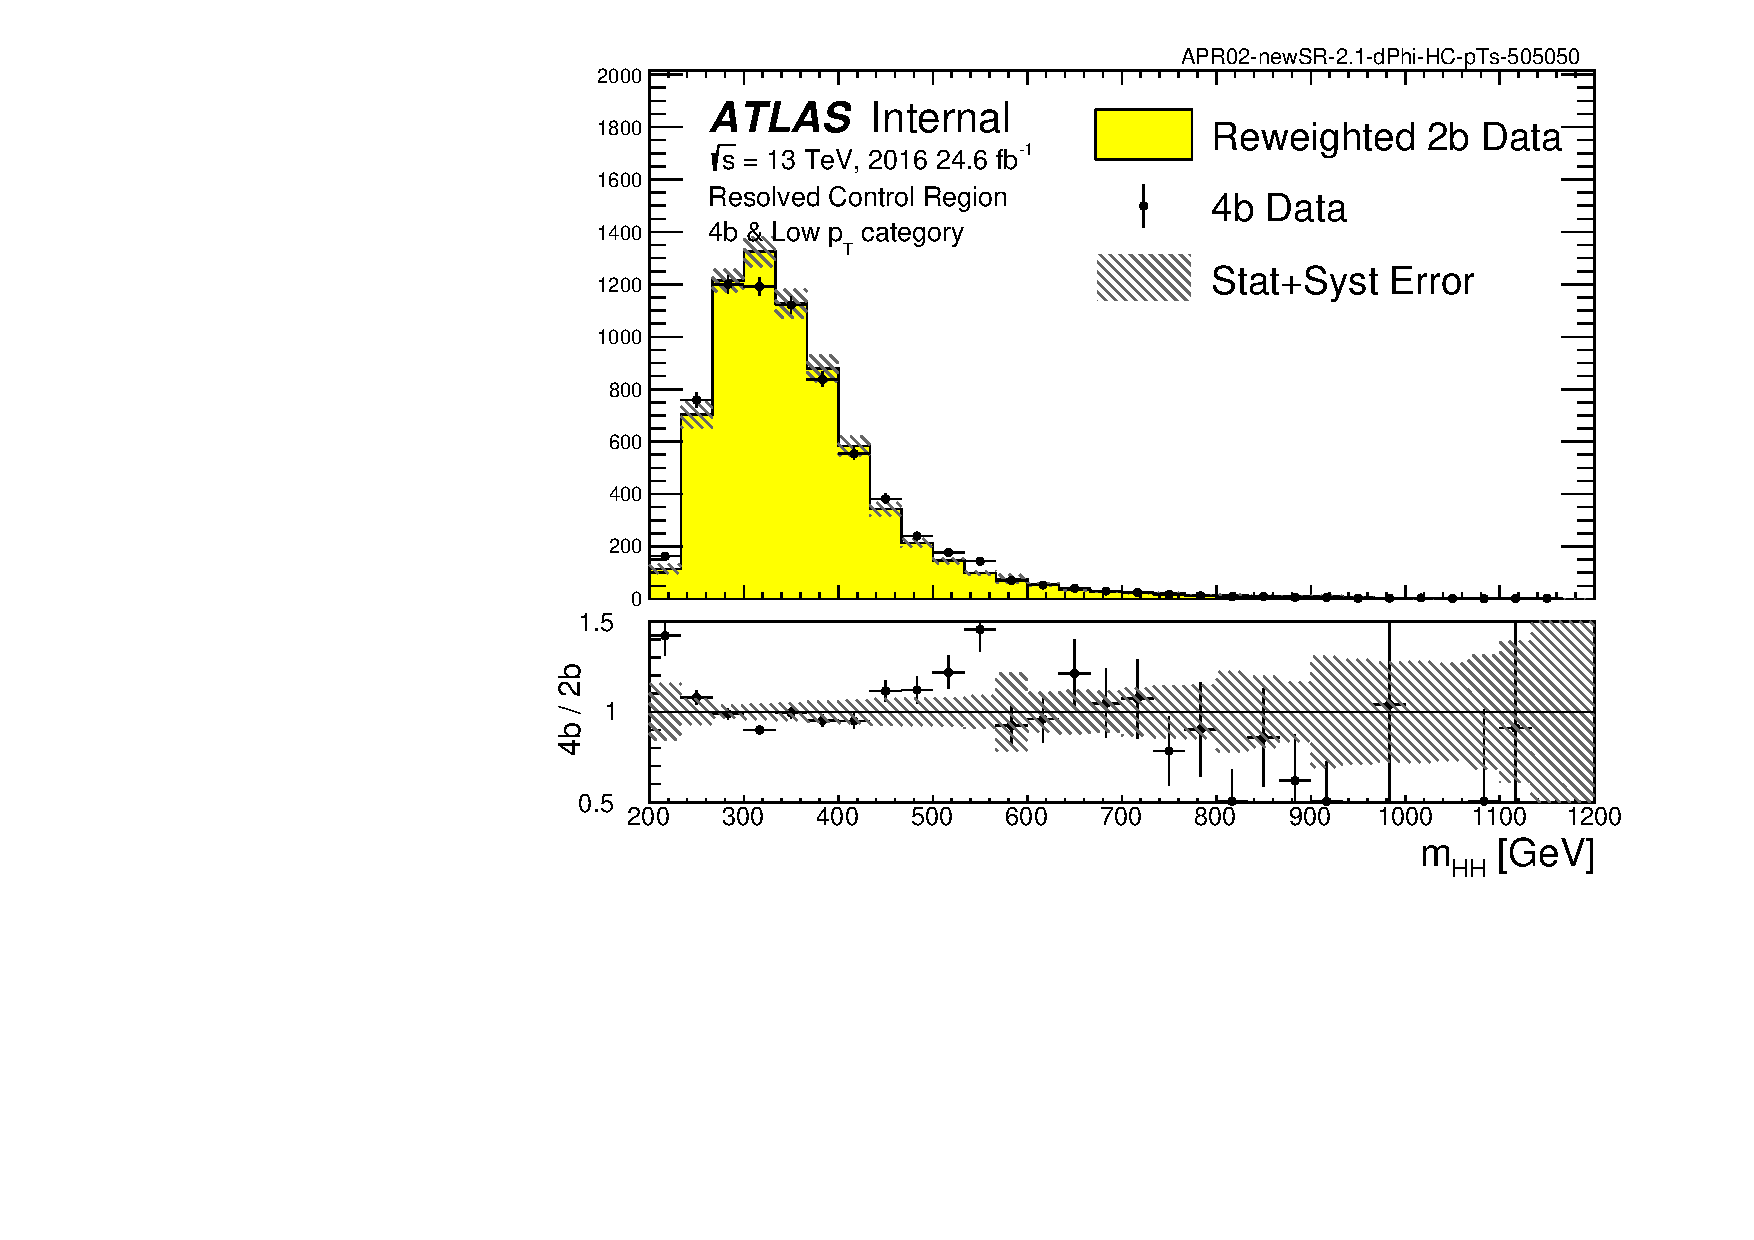
\includegraphics[width=0.4\textwidth]{\figpath{bkgdest-strategy/2016/bkgdest-m-hh-bstrap-med-shapesyst-Control-4bLowPtcat-NN-16.pdf}}
    }
    \caption{Distributions of $m_{\higgs\higgs}$ before and after reweighting, which includes log(pt)-s of the 1st and 3rd Higgs candidate jets, in the 2016 Control Region.}
    \label{fig:bkgdest16-5-Control-4bLowPtcat}
\end{figure}


